%%%%%%%%%%%%%%%%%%%%%%%%%%%%%%%%%%%%%%%%%%%%%%%%%%%%%%%%%%%%%%%%%%%%%%
% LaTeX Example: Project Report
%
% Source: http://www.howtotex.com
%
% Feel free to distribute this example, but please keep the referral
% to howtotex.com
% Date: March 2011 
% 
%%%%%%%%%%%%%%%%%%%%%%%%%%%%%%%%%%%%%%%%%%%%%%%%%%%%%%%%%%%%%%%%%%%%%%

\documentclass[paper=letter, fontsize=11pt]{article}
\usepackage[T1]{fontenc}
\usepackage{fourier}

\usepackage[english]{babel}															% English language/hyphenation
%\usepackage[protrusion=true,expansion=true]{microtype}	
\usepackage{amsmath,amsfonts,amsthm} % Math packages
\usepackage[pdftex]{graphicx}	
\usepackage{url}
\usepackage{siunitx}
\usepackage{subfig}
\usepackage{pgf}
\usepackage{float}



%%% Custom sectioning
\usepackage{sectsty}
\allsectionsfont{ \normalfont\scshape}


%%% Custom headers/footers (fancyhdr package)
\usepackage{fancyhdr}
\pagestyle{fancyplain}
\fancyhead{}											% No page header
\fancyfoot[L]{}											% Empty 
\fancyfoot[C]{}											% Empty
\fancyfoot[R]{\thepage}									% Pagenumbering
\renewcommand{\headrulewidth}{0pt}			% Remove header underlines
\renewcommand{\footrulewidth}{0pt}				% Remove footer underlines
\setlength{\headheight}{13.6pt}


%%% Equation and float numbering
\numberwithin{equation}{section}		% Equationnumbering: section.eq#
\numberwithin{figure}{section}			% Figurenumbering: section.fig#
\numberwithin{table}{section}				% Tablenumbering: section.tab#


%%% Maketitle metadata
\newcommand{\horrule}[1]{\rule{\linewidth}{#1}} 	% Horizontal rule

\title{
		%\vspace{-1in} 	
		\usefont{OT1}{bch}{b}{n}
		\normalfont \normalsize \textsc{State University at Buffalo} \\ [25pt]
		\horrule{0.5pt} \\[0.4cm]
		\Large Project 2 : Clustering Algorithm \\
		\horrule{2pt} \\[0.5cm]
}
\author{
		\normalfont\large 								
        Yuze Liu \hspace{0.6cm}50207903\\
        \normalfont\large 
        Luting Chen \hspace{0.5cm}50133507\\
        \normalfont\large 
        Vicky Zheng \hspace{0.5cm}50037709\\
}
\date{\large 11/04/2016}
%%% Begin document
\begin{document}
\maketitle
%\newdimen\origiwspc%
\section{K-Means Algorithm}
\subsection{Algorithm Description}
K Means clustering is a method of vector quantization. K-means clustering aims to partition n observations into k clusters in which each observation belongs to the cluster with the nearest mean.
\subsection{Implementation}
In the clustering problem, we are given a data set $x^{(1)},...,x^{(m)}$, and want to group the data into a few cohesive "clusters." Here, we are given feature vectors for each data point $x^{(i)} \in Dataset$; Our goal is to predict $k$ centroids and a label $c^{(i)}$ for each data point.\\ 
The pseudo code for K-Means Algorithm is as follows:\\
\begin{enumerate}
	\item Initialize cluster centroid $\mu_1,\mu_2,\mu_3,...\mu_k \in DataSet$
	\item Repeat until converge: \{\\
	      \hspace*{0.5cm}for every $i$, set:\\
	      \hspace*{0.9cm}$c^{(i)} :=$ arg min $||x^{(i)} - \mu_j||^2$\\
	      \hspace*{0.5cm}for each j, set :\\
	      \hspace*{0.9cm}$\mu_j := \frac{\Sigma_{m-1}^{m} \{c^{(i)} = j\}x^{(i)}}{\Sigma_{m-1}^{m}\{c^{(i)} = j\}}$\\
	\}
\end{enumerate}
So for each iteration, we assign the data point to the nearest center, this way, a new cluster will be formed. For each cluster, we then calculate the new center for them, we repeat this procedure until the cluster is no longer changed.\\
In the program, we first randomly picked K points from the dataset as the initial center. We used build in random function from python, each time we run the code, the initial center will be different, this will have a effect with the result. But to compare the result from K-Means and MapReduce K-Means, we used random.seed() function, to make sure the initial center is the same for both program for this single run.\\
\subsection{Result Visualization}
We have been provided with 4 dataset,'cho.txt', 'iyer.txt', 'new\_dataset\_1.txt', and 'new\_dataset\_2.txt'. Here is the result for each dataset. Since the ground truth cluster has been provided in the dataset, so we we choose how many clusters we need for this dataset, we just use the number of ground truth clusters.\\
For the data that has outliers, we didn't remove them before running the program. But when we calculate the external index, we have deleted the outliers from the dataset.\\
\noindent Rand Index = 0.7542\\
Jaccard Coefficient = 0.2953\\
\begin{figure}[H]
	\centering
	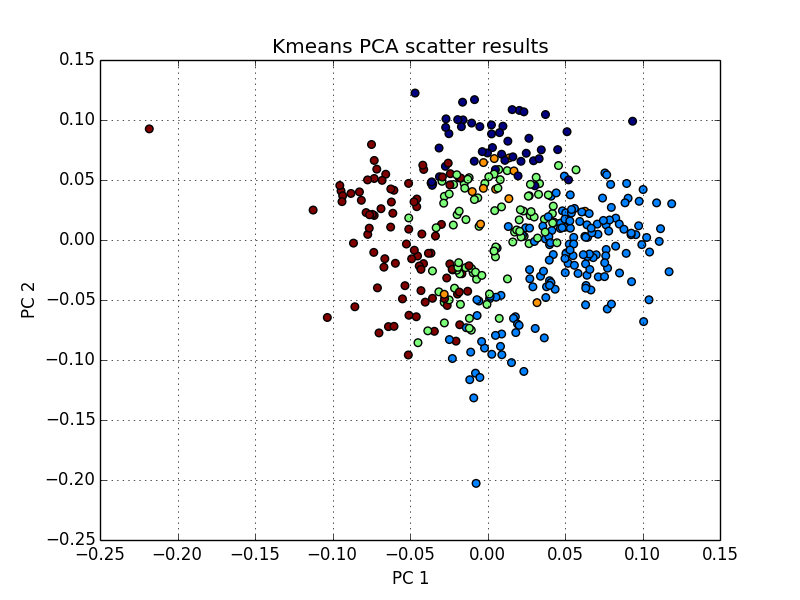
\includegraphics[width=0.8\textwidth]{K_cho_2D}
	\caption{Result of K\_Means Algorithm on Cho DataSet 2D Version, K=5}
\end{figure}
\begin{figure}[H]
	\centering
	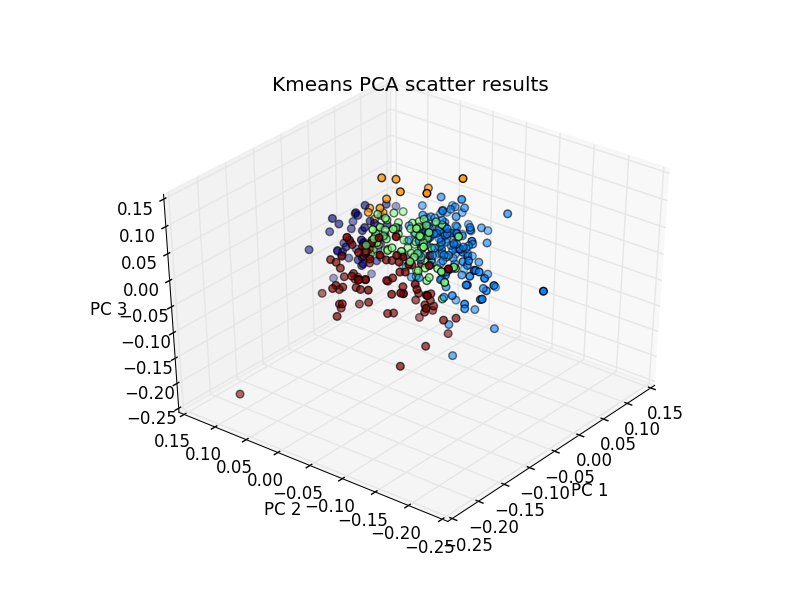
\includegraphics[width=0.8\textwidth]{K_cho_3D}
	\caption{Result of K\_Means Algorithm on Cho DataSet 3D Version, K=5}
\end{figure}
\noindent Rand Index = 0.8140\\
Jaccard Coefficient = 0.2543\\
\begin{figure}[H]
	\centering
	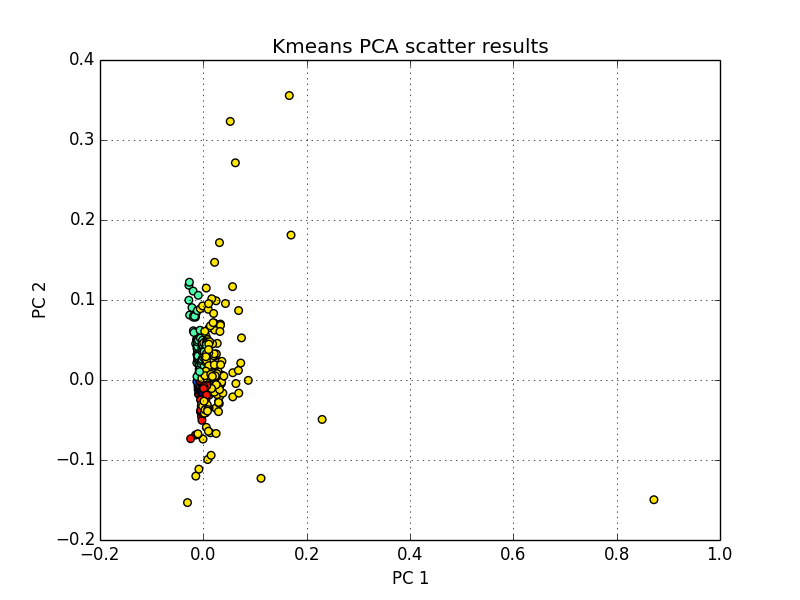
\includegraphics[width=0.8\textwidth]{K_iyer_2D}
	\caption{Result of K\_Means Algorithm on iyer DataSet 2D Version,K=10}
\end{figure}
\begin{figure}[H]
	\centering
	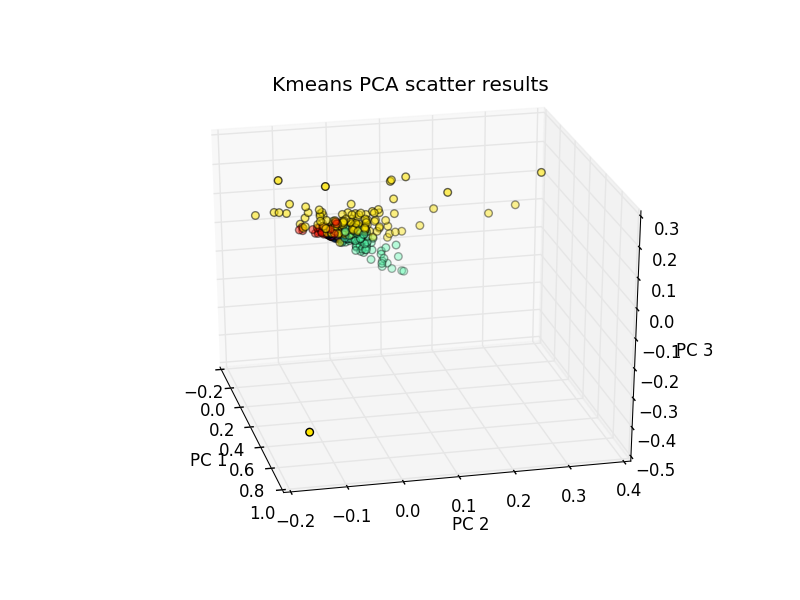
\includegraphics[width=0.8\textwidth]{K_iyer_3D}
	\caption{Result of K\_Means Algorithm on iyer DataSet 3D Version,K=10}
\end{figure}
\noindent Rand Index = 0.7330\\
Jaccard Coefficient = 0.5194\\
\begin{figure}[H]
	\centering
	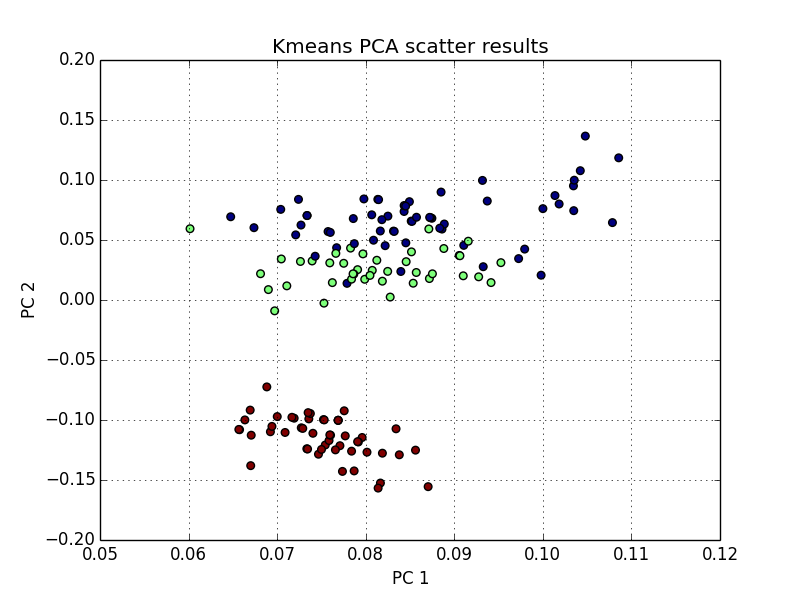
\includegraphics[width=0.8\textwidth]{K_new_dataset_1_2D}
	\caption{Result of K\_Means Algorithm on new dataset1 2D Version,K=3}
\end{figure}
\begin{figure}[H]
	\centering
	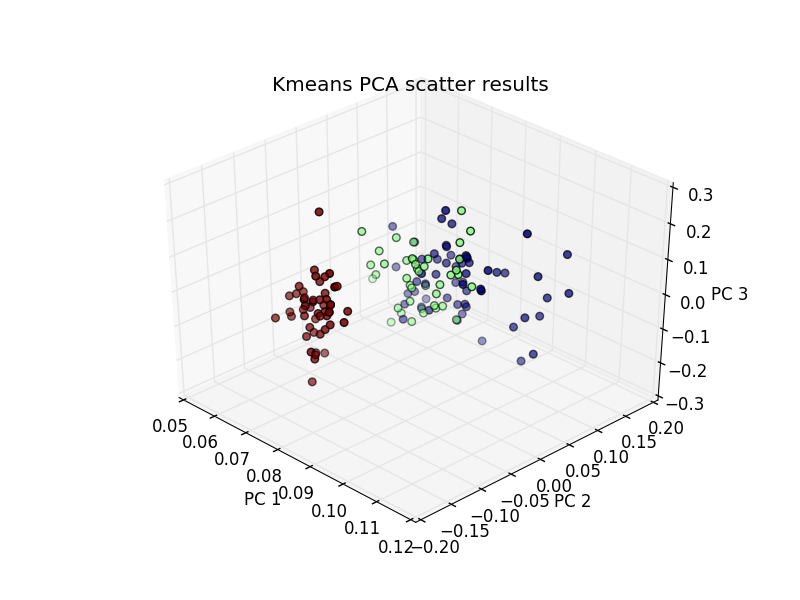
\includegraphics[width=0.8\textwidth]{K_new_dataset_1_3D}
	\caption{Result of K\_Means Algorithm on new dataset1 3D Version,K=3}
\end{figure}
\noindent Rand Index = 1\\
Jaccard Coefficient = 1\\
\begin{figure}[H]
	\centering
	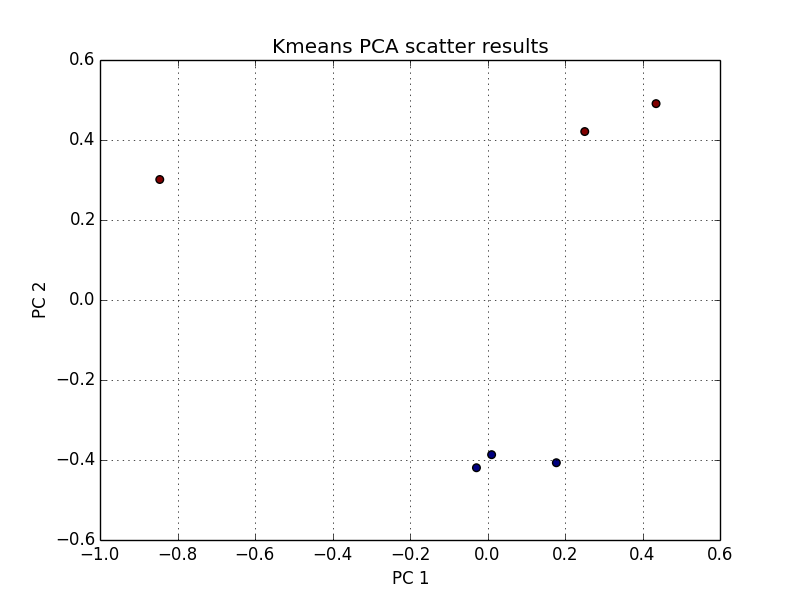
\includegraphics[width=0.8\textwidth]{K_new_dataset_2_2D}
	\caption{Result of K\_Means Algorithm on new dataset2 3D Version,K=2}
\end{figure}
\begin{figure}[H]
	\centering
	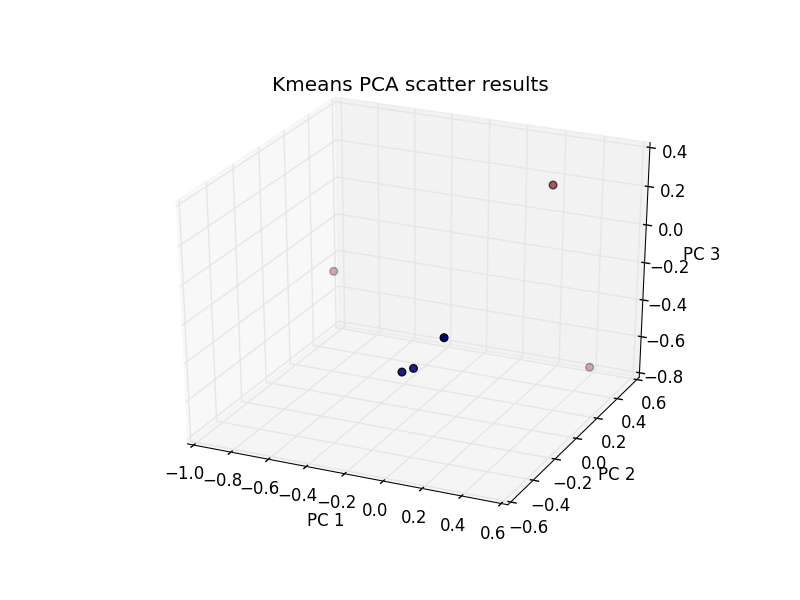
\includegraphics[width=0.8\textwidth]{K_new_dataset_2_3D}
	\caption{Result of K\_Means Algorithm on new dataset2 3D Version,K=2}
\end{figure}
\subsection{Result Evaluation}
The result of K-Means is highly related to the initial K centers we chose. \\
For the dataset2, it's the simplest dataset among these 4 datasets. The result is good, both the rand index and the Jaccard Coefficient are both 1. But during several runs, it still has the choice to get lower value because the selection of the initial centers are random.\\
The advantage of the K-means:\\
1. Compare to other algorithm, the K-Means runs really fast and can be guaranteed to converge. Especially when the dataset is huge and we keep the k in a reasonable amount, the algorithm runs very fast. \\
2. K-Means produce tighter clusters than Hierarchical clustering. 
The disadvantage of the K-means:\\
1. It's difficult to predict K value. For this project, since we already know the ground truth result, so we can choose the right K for each dataset. But in the reality, for a given dataset, we can't know the proper value of K, so we need to predict K, which makes it hard.\\
2. Different initial centers can result in different final clusters\\
3. If the dataset has outliers, it will be hard to get the outliers out of the data. And if one of the outliers has been chosen as the initial center, then it will yield bad result.\\
\section{Hierarchical Agglomerative Clustering}
\subsection{Algorithm Description}
In hierarchical  agglomerative clustering, we build a hierarchy of clusters in a bottom-up fashion. To begin with, each observation is treated as a cluster, giving us N clusters if we have N observations at hand. Then we merge pairs of clusters while moving up the hierarchy, in the end we have the root of the hierarchy, which contains all observations in one cluster. The merging policy is greedy: each time, we only merge the pair of clusters that has the smallest inter-cluster distance according to some dissimilarity function.
\subsection{Implementation}
Some important variables and data structures:\\
ids : the list of observation IDs;\\
gts: the list of observation ground truth;\\
ges: the matrix of observation features;\\
cluster\_list: the list of all appearing clusters in the hierarchy;\\
p\_dist: the matrix of pairwise Euclidean distance for observations\\


We write 2 functions for the purpose of hierarchical clustering: 
\begin{enumerate}
	\item res = hierarchical\_clustering(p\_dist)
	\item clustering = hc\_cluster\_n(cluster\_num,res)
\end{enumerate}

Function hierarchical\_clustering(p\_dist) returns the whole hierarchy using global variables ids, ges, clustering\_list and p\_dist.
Function hc\_cluster\_n(cluster\_num,res) returns and prints the list of cluster labels after passing cluster\_num(the number of clusters) and res(the whole cluster hierarchy)


For cluster dissimilarity, we use Euclidean distance to compute the dissimilarity between observations and use Single linkage as our linkage criteria. 

We use a python list named  cluster\_list to store all clusters appearing in the hierarchy, each element in cluster\_list is one cluster, which contains the IDs of observation members. The hierarchy is also stored in a list and one level of the hierarchy is one element of the list. The following is an example.

\begin{figure}[H]
	\centering
	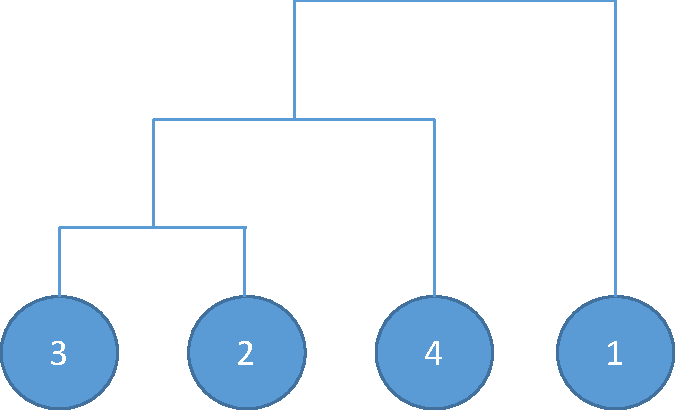
\includegraphics[width=0.8\textwidth]{example_den.pdf}
	\caption{Dendrogram of a toy example with 4 points}
\end{figure}

\begin{figure}[H]
	\centering
	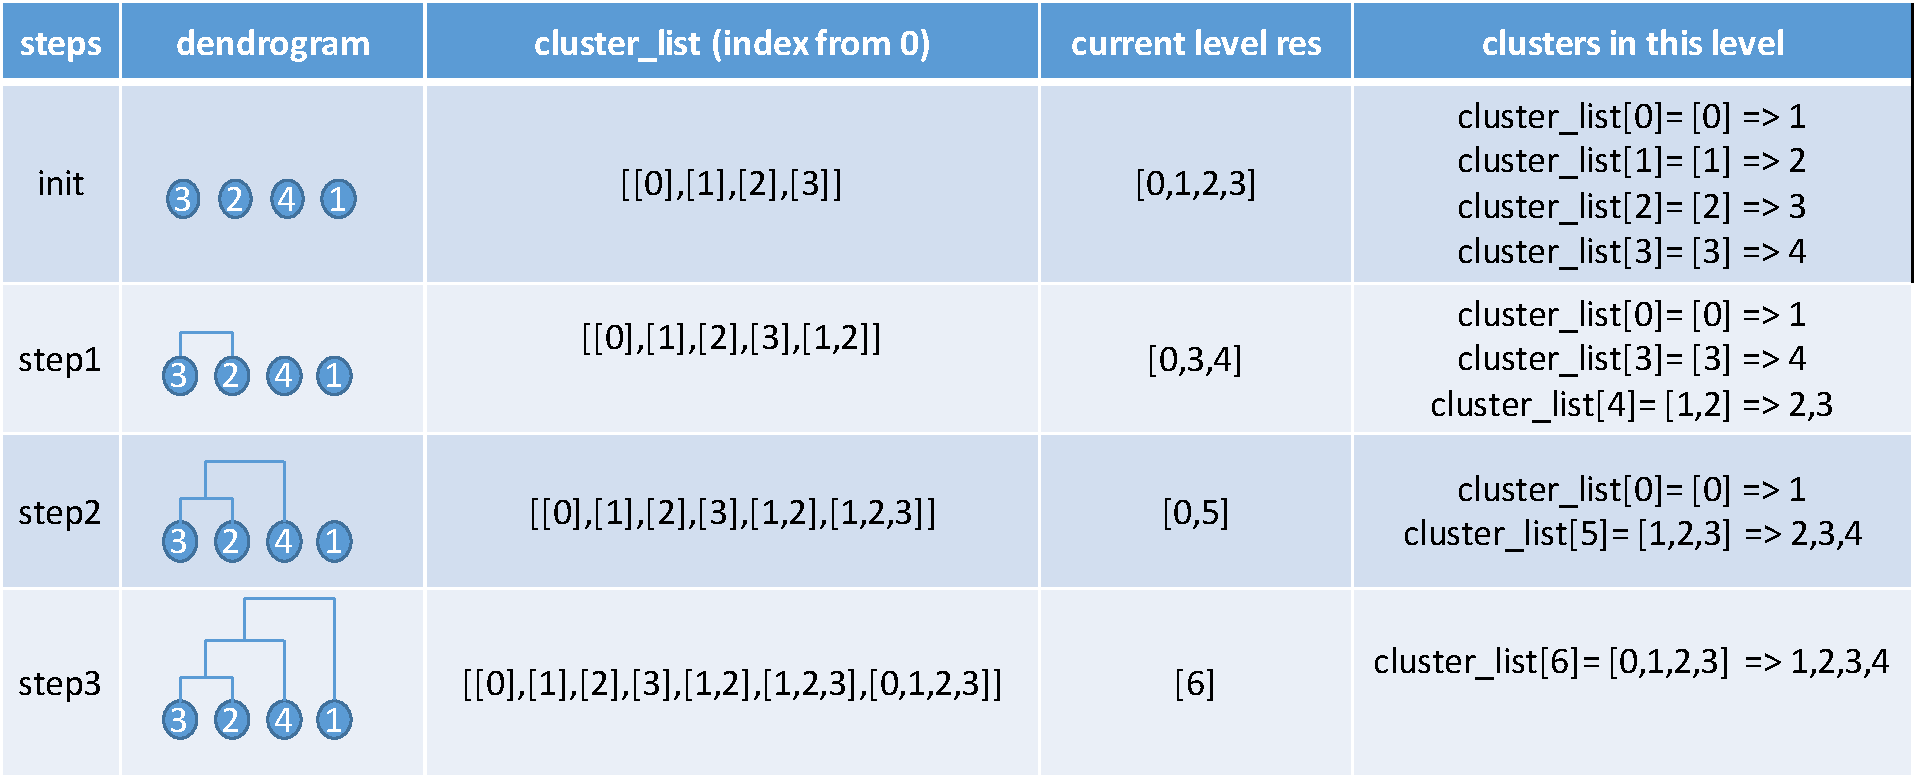
\includegraphics[width=0.8\textwidth]{example_table.pdf}
	\caption{ Steps of hierarchical agglomerative clustering for the toy example}
\end{figure}


\subsection{Result Visualization}
\begin{figure}[H]
	\centering
	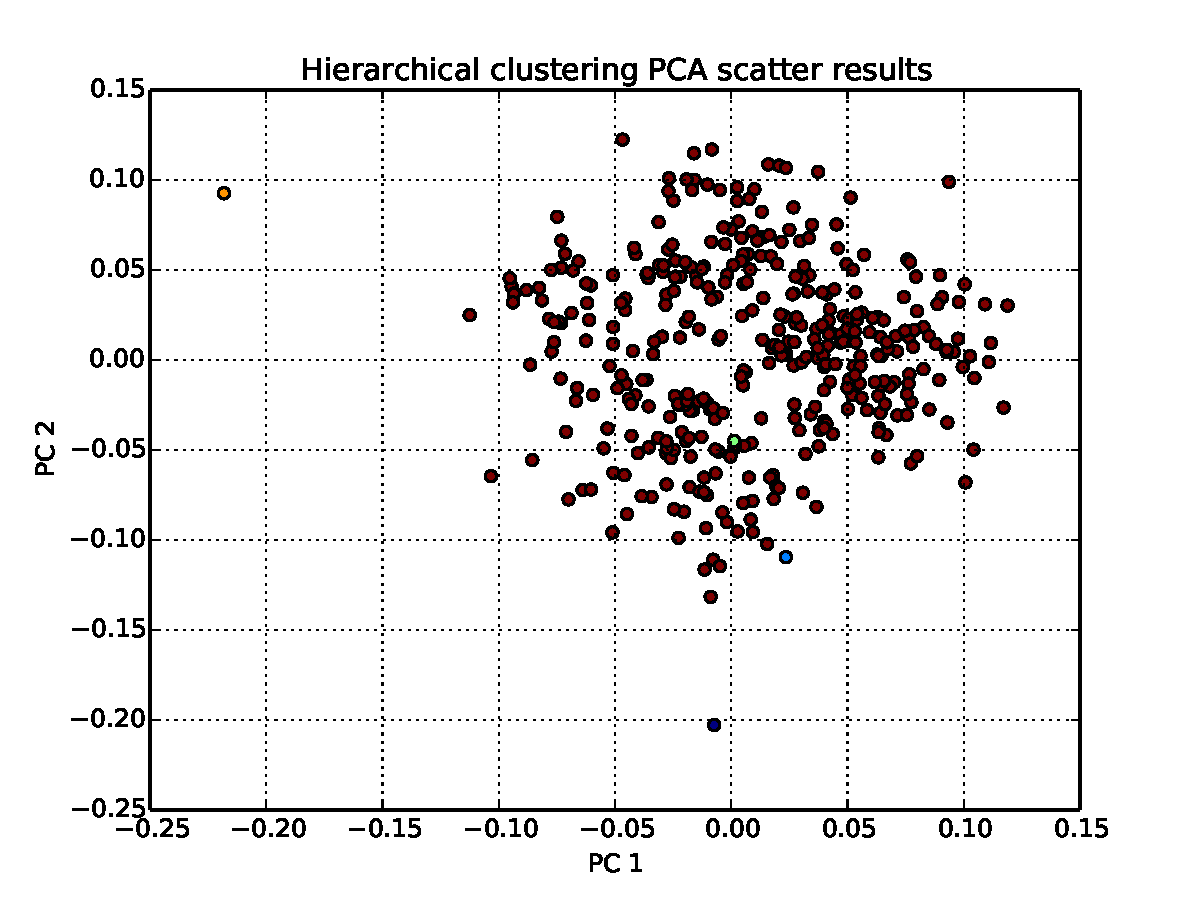
\includegraphics[width=0.8\textwidth]{H_cho_2D.pdf}
	\caption{Result of hierarchical clustering on Cho DataSet 2D Version, K=5}
\end{figure}

\begin{figure}[H]
	\centering
	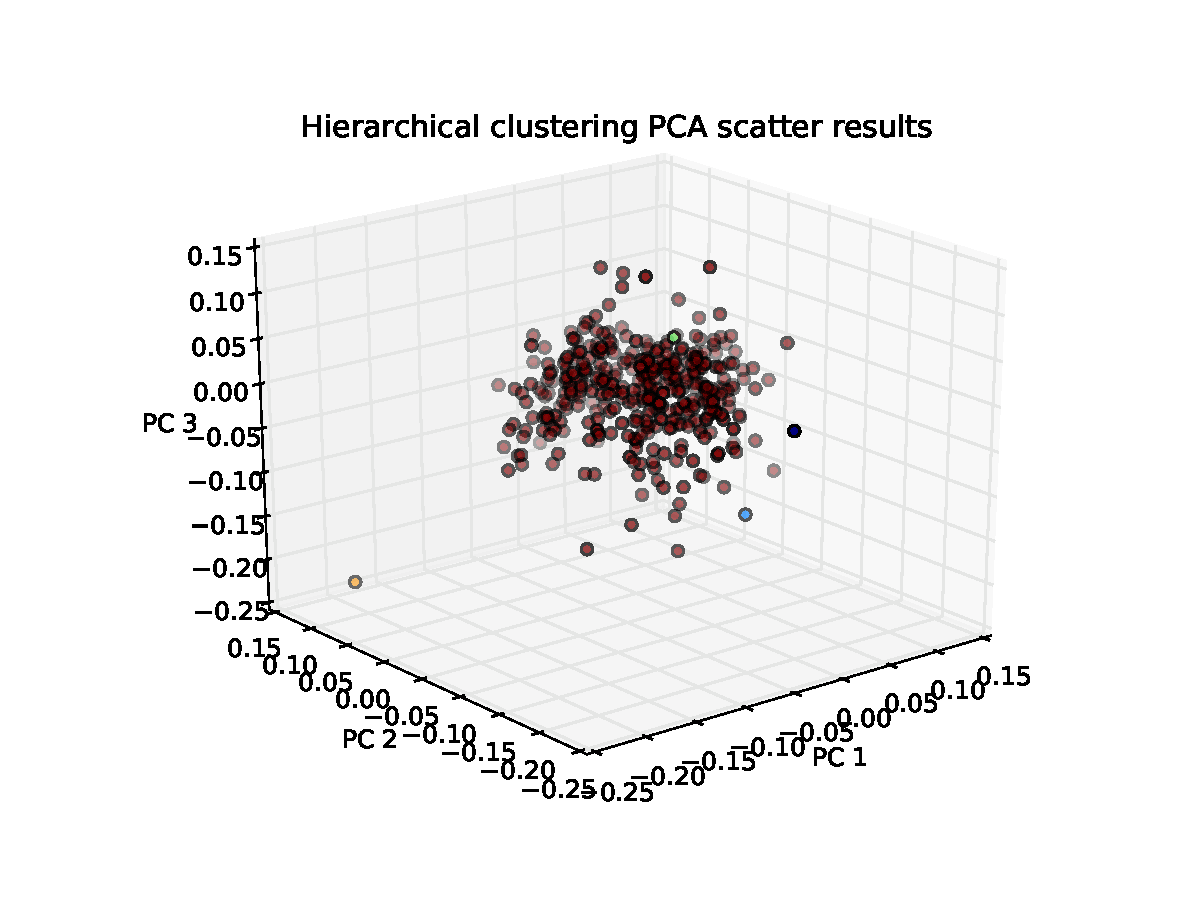
\includegraphics[width=0.8\textwidth]{H_cho_3D.pdf}
	\caption{Result of hierarchical clustering on Cho DataSet 3D Version, K=5}
\end{figure}
\noindent Rand Index = 0.2403\\
Jaccard Coefficient = 0.2284\\

\begin{figure}[H]
	\centering
	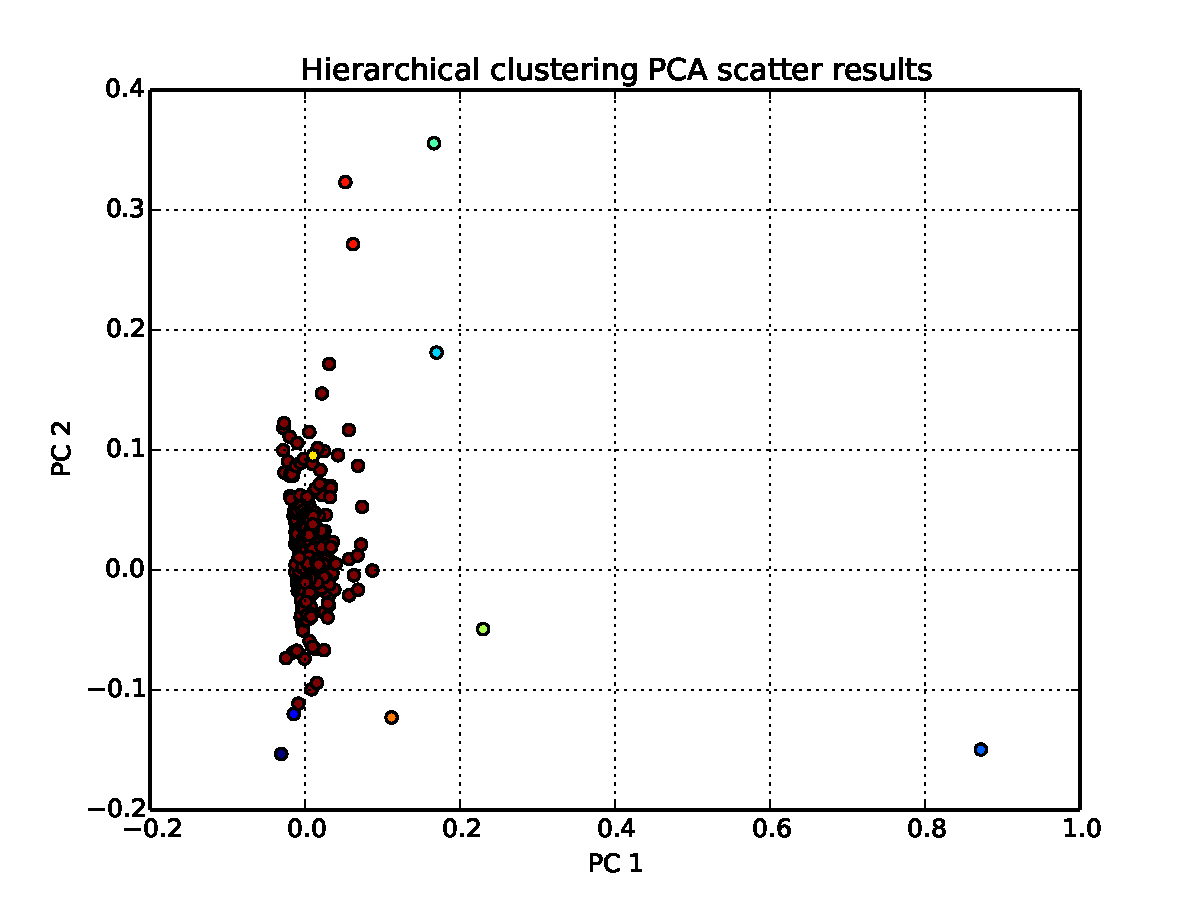
\includegraphics[width=0.8\textwidth]{H_iyer_2D.pdf}
	\caption{Result of hierarchical clustering on Iyer DataSet 2D Version, K=10}
\end{figure}

\begin{figure}[H]
	\centering
	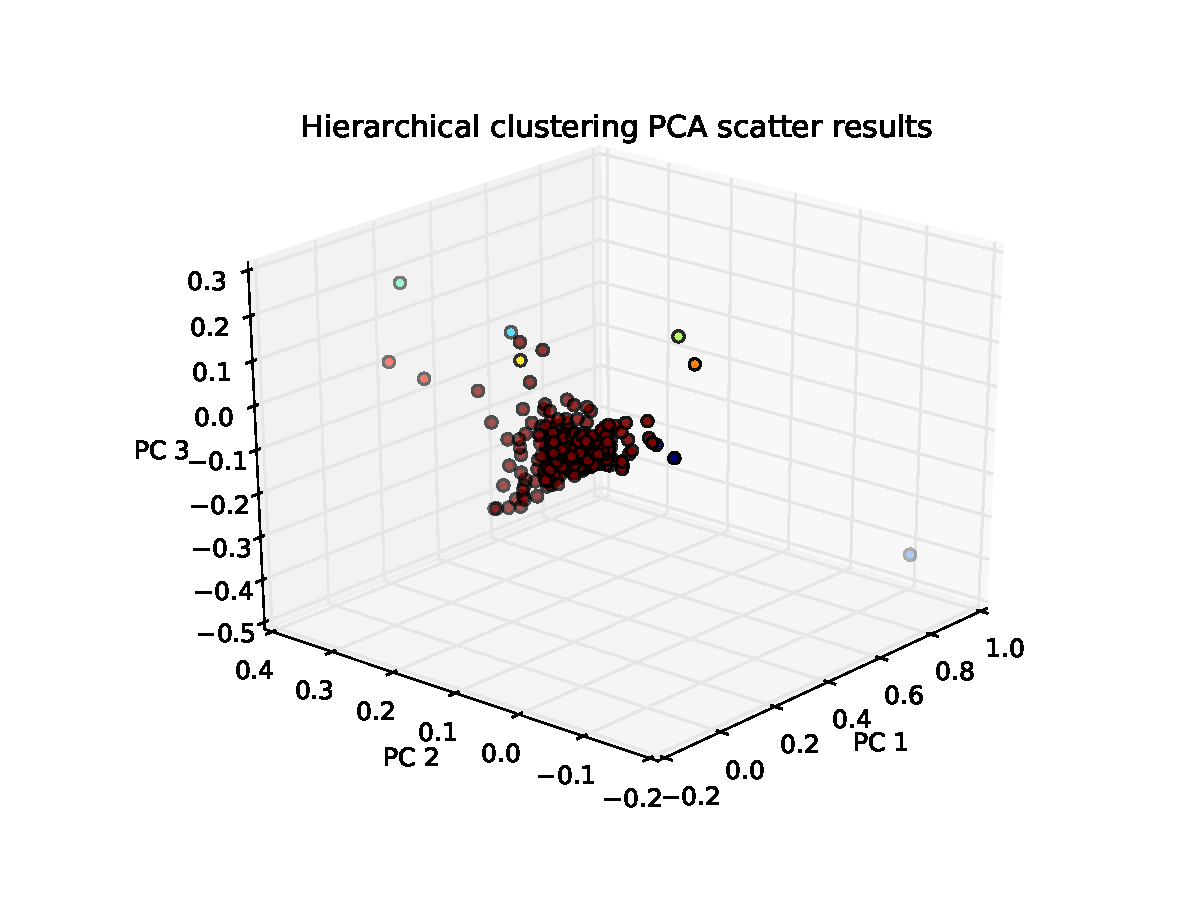
\includegraphics[width=0.8\textwidth]{H_iyer_3D.pdf}
	\caption{Result of hierarchical clustering on Iyer DataSet 3D Version, K=10}
\end{figure}
\noindent Rand Index = 0.2074\\
Jaccard Coefficient = 0.1761\\

\begin{figure}[H]
	\centering
	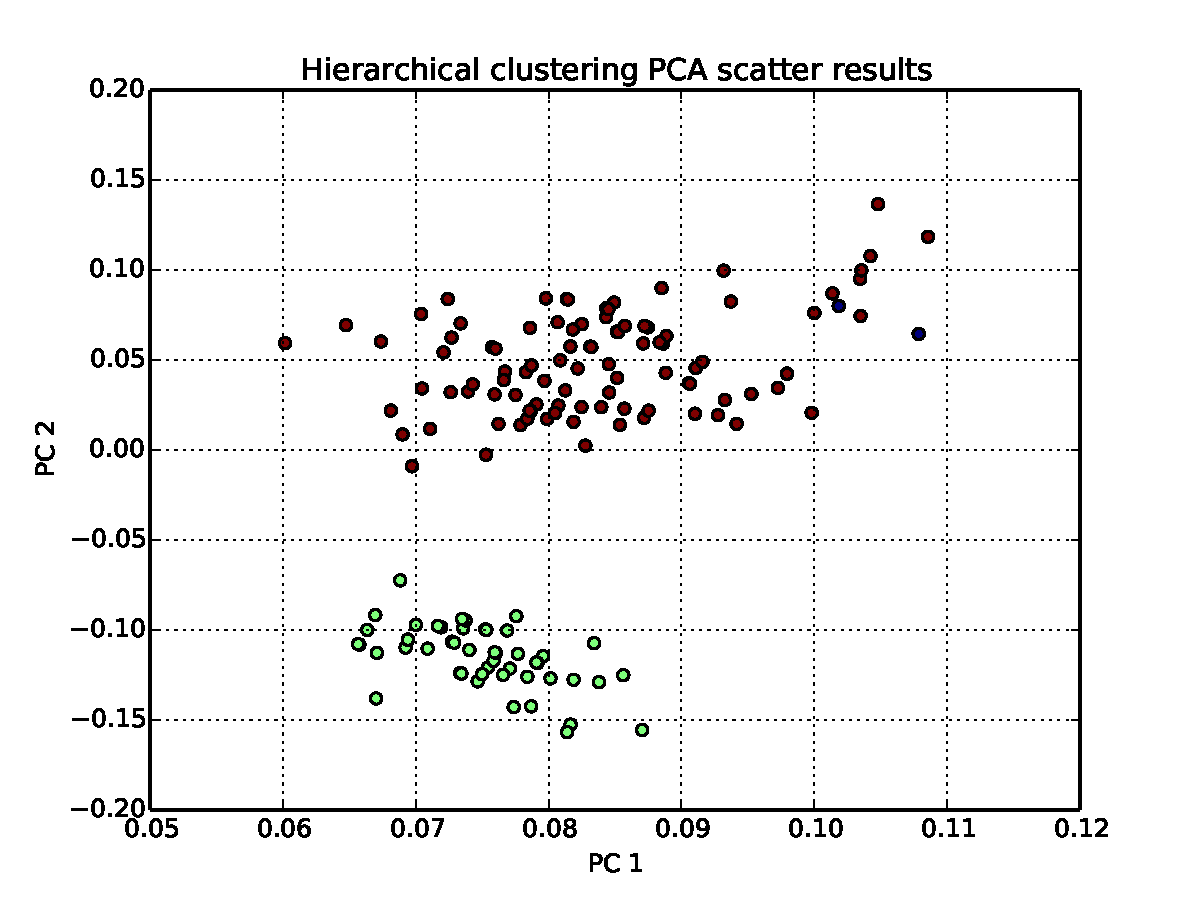
\includegraphics[width=0.8\textwidth]{H_new_dataset_1_2D.pdf}
	\caption{Result of hierarchical clustering on new DataSet  1 2D Version, K=3}
\end{figure}

\begin{figure}[H]
	\centering
	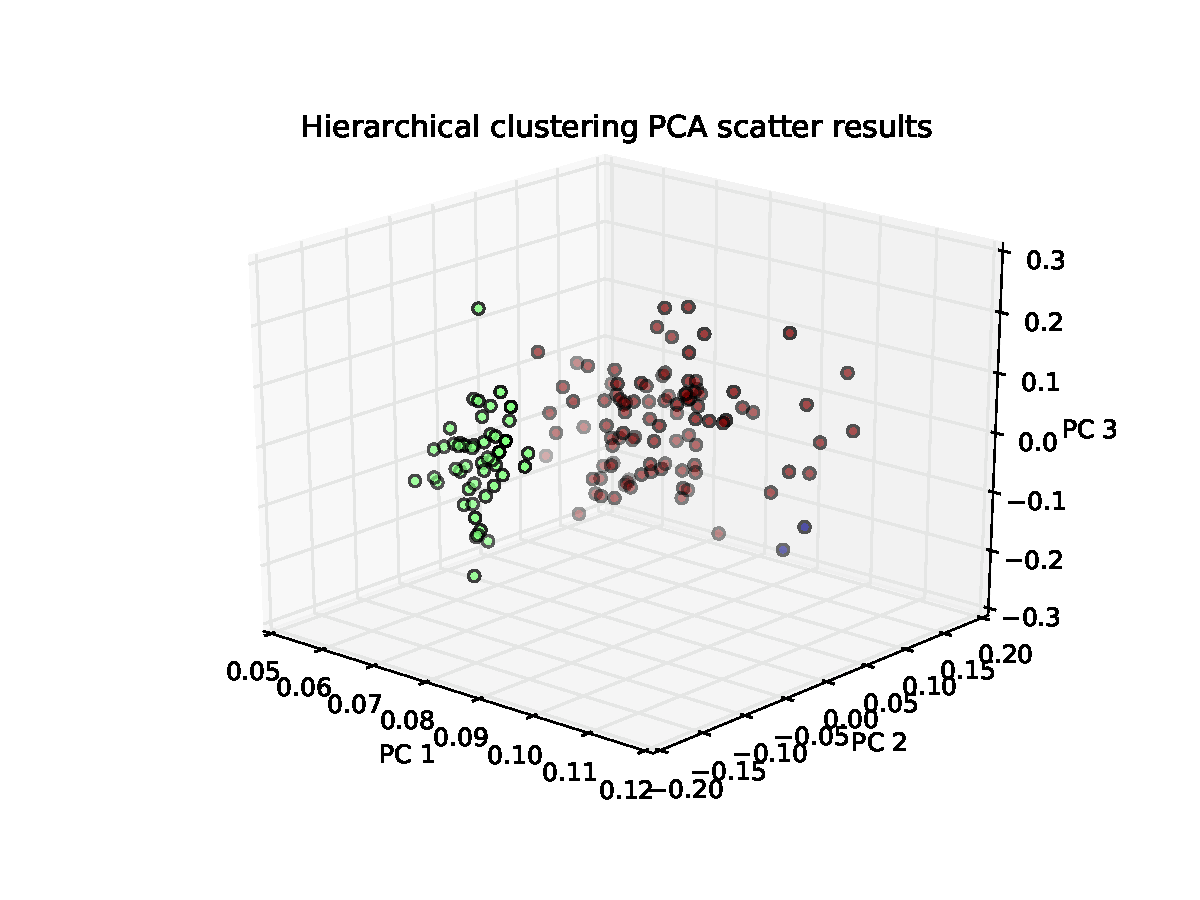
\includegraphics[width=0.8\textwidth]{H_new_dataset_1_3D.pdf}
	\caption{Result of hierarchical clustering on new DataSet 1 3D Version, K=3}
\end{figure}
\noindent Rand Index = 0.7781\\
Jaccard Coefficient = 0.5941\\


\begin{figure}[H]
	\centering
	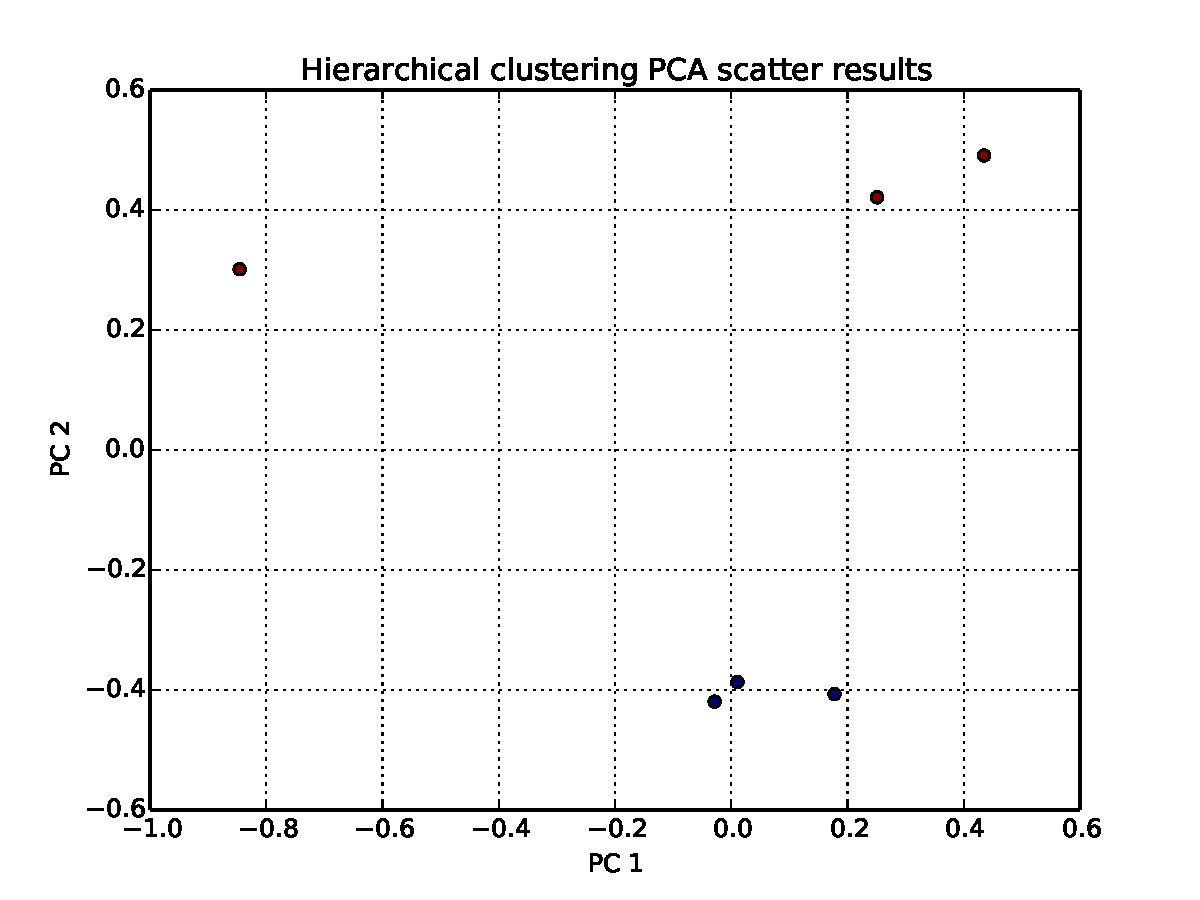
\includegraphics[width=0.8\textwidth]{H_new_dataset_2_2D.pdf}
	\caption{Result of hierarchical clustering on new DataSet 2 2D Version, K=2}
\end{figure}

\begin{figure}[H]
	\centering
	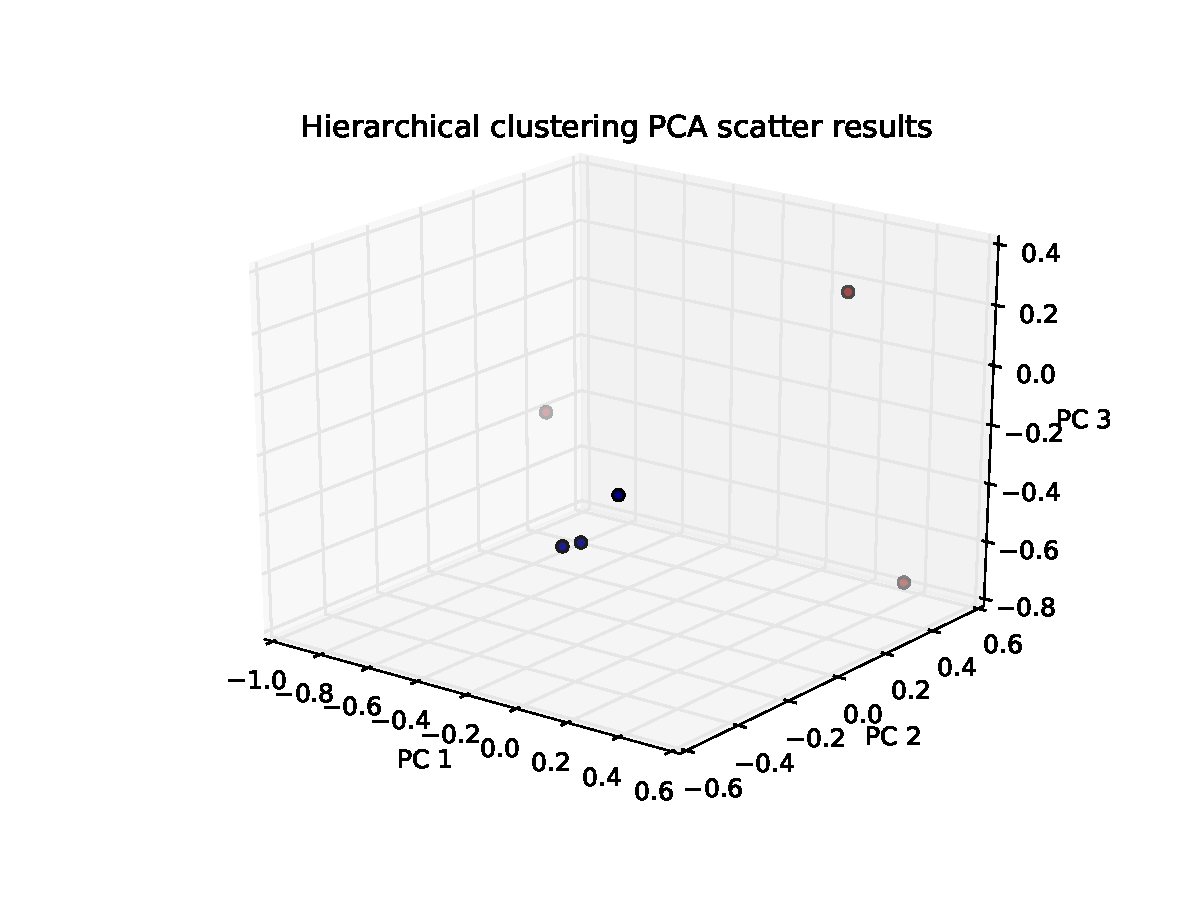
\includegraphics[width=0.8\textwidth]{H_new_dataset_2_3D.pdf}
	\caption{Result of hierarchical clustering on new DataSet 2 3D Version, K=2}
\end{figure}
\noindent Rand Index = 1.0000\\
Jaccard Coefficient = 1.0000\\

\subsection{Result Evaluation}
Here we are asked to use single linkage, so it will merge 2 clusters if they have the pair of points that has the smallest distance. One drawback of the algorithm is that it doesn't take into consideration the positions of other points in the clusters. The cho dataset shows the drawback of  hierarchical clustering clearly. It contain some points that are far away from the other points, so they will be merged in the last few steps and hence more likely to become clusters with one single point.  And it's also slower compared to other algorithms.

Some advantages of hierarchical clustering are it builds the dendrogram and can yield results for different cluster numbers easily; besides, it doesn't need to specify the number of clusters.

\section{Spectral Algorithm}
\subsection{Algorithm Description}
Spectral clustering computes a low-dimension embedding of the affinity matrix between samples, and then it performs K\_Means in the low dimensional space and uses the resulting cluster labels as final results.
\subsection{Implementation}
We follow the pipeline by \cite{sp_clustering}. The following is the details.

\begin{figure}[H]
	\centering
	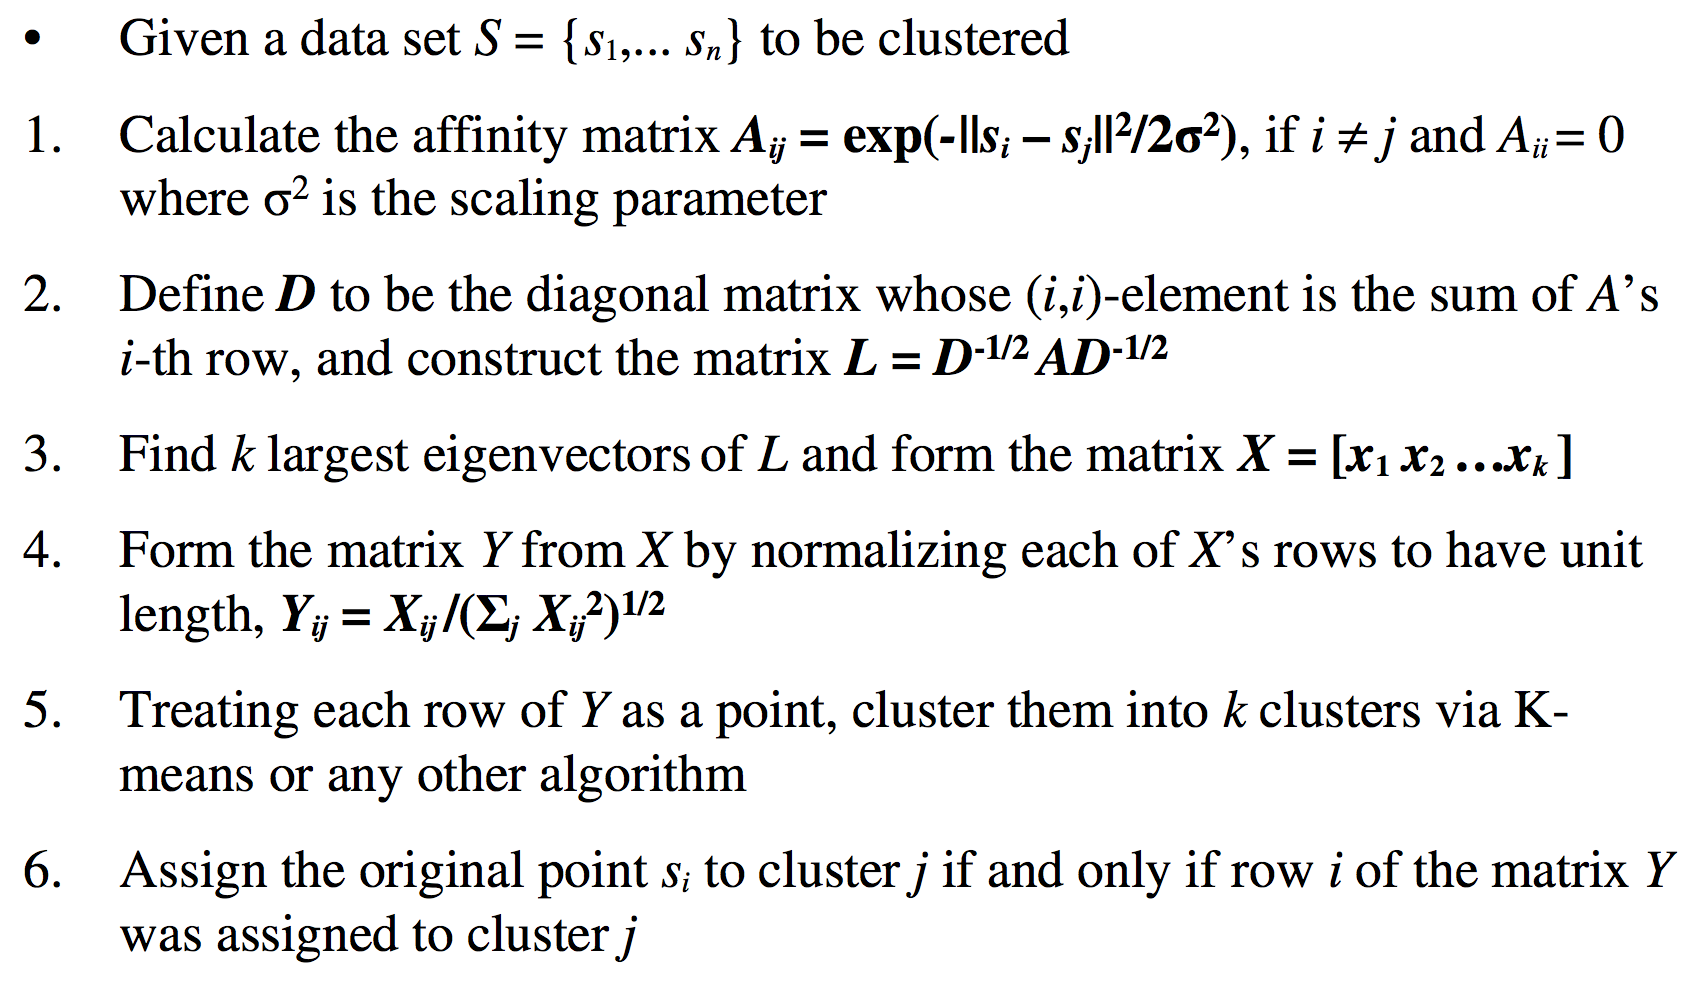
\includegraphics[width=0.8\textwidth]{sp_pipeline.png}
	\caption{Pipeline for spectral clustering }
\end{figure}

To notice, laplace matrix L has many forms. Instead of using L defined in class slides, we follow the definition of \cite{sp_clustering}, where  $L= D^{-0.5}AD^{-0.5}$ instead of using $L_{slide}= D^{-0.5}(D-A)D^{-0.5}$. Their relationship is easy to get: $L_{slide}= D^{-0.5}(D-A)D^{-0.5}= I - D^{-0.5}AD^{-0.5} = I - L$ and eigen values of our L equals to 1 minus the corresponding eigen values of $L_{slide}$. So here we choose the k eigen vectors corresponding to the k largest eigen values. In our program, we can specify the value of  $\sigma$,  or we can choose  optimal $\sigma$ automatically by searching over candidates of $\sigma$s and choose the one that yields highest external index value. In our implementation, we use rand index for default to judge if one $\sigma$ is good.   
\subsection{Result Visualization}

\begin{figure}[H]
	\centering
	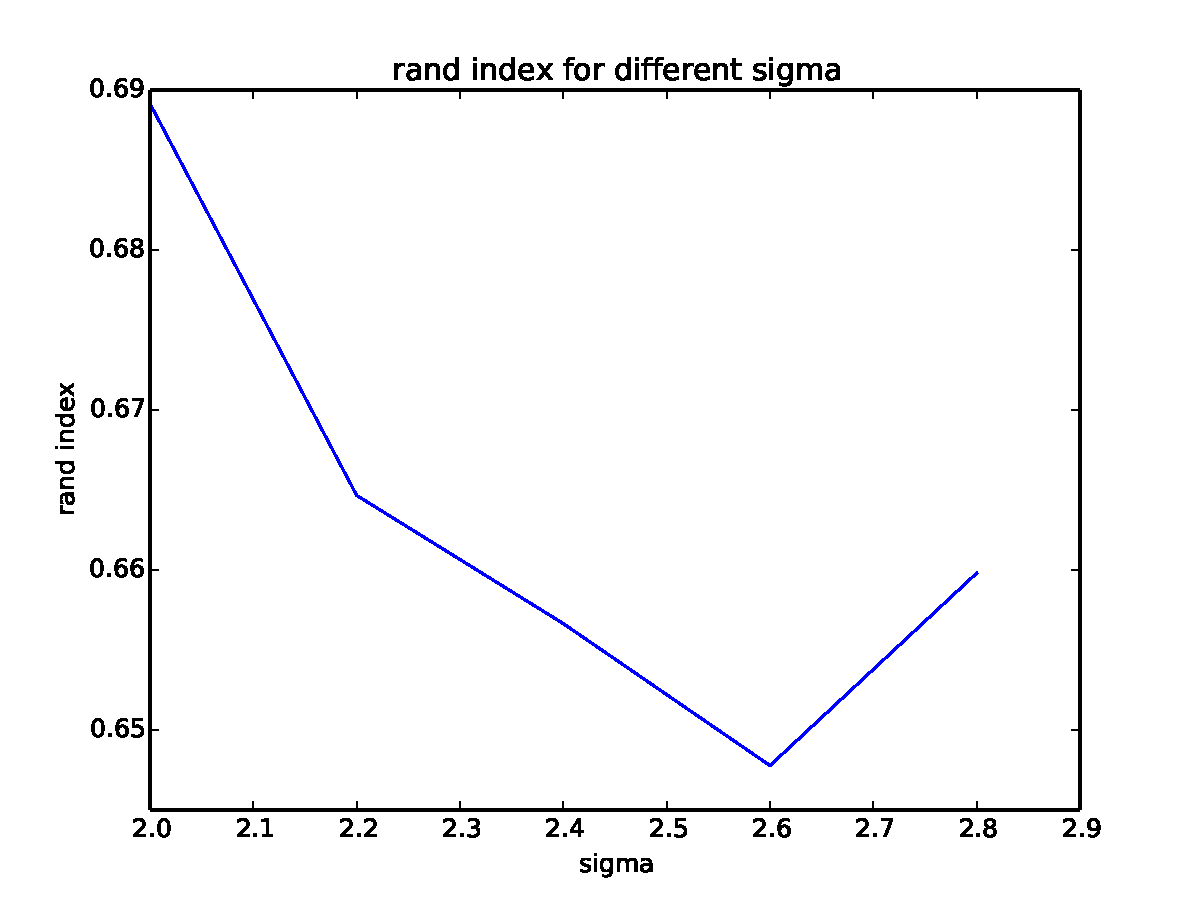
\includegraphics[width=0.8\textwidth]{choose_sigma_cho.pdf}
	\caption{Choosing $\sigma$ for Cho DataSet  }
\end{figure}


\begin{figure}[H]
	\centering
	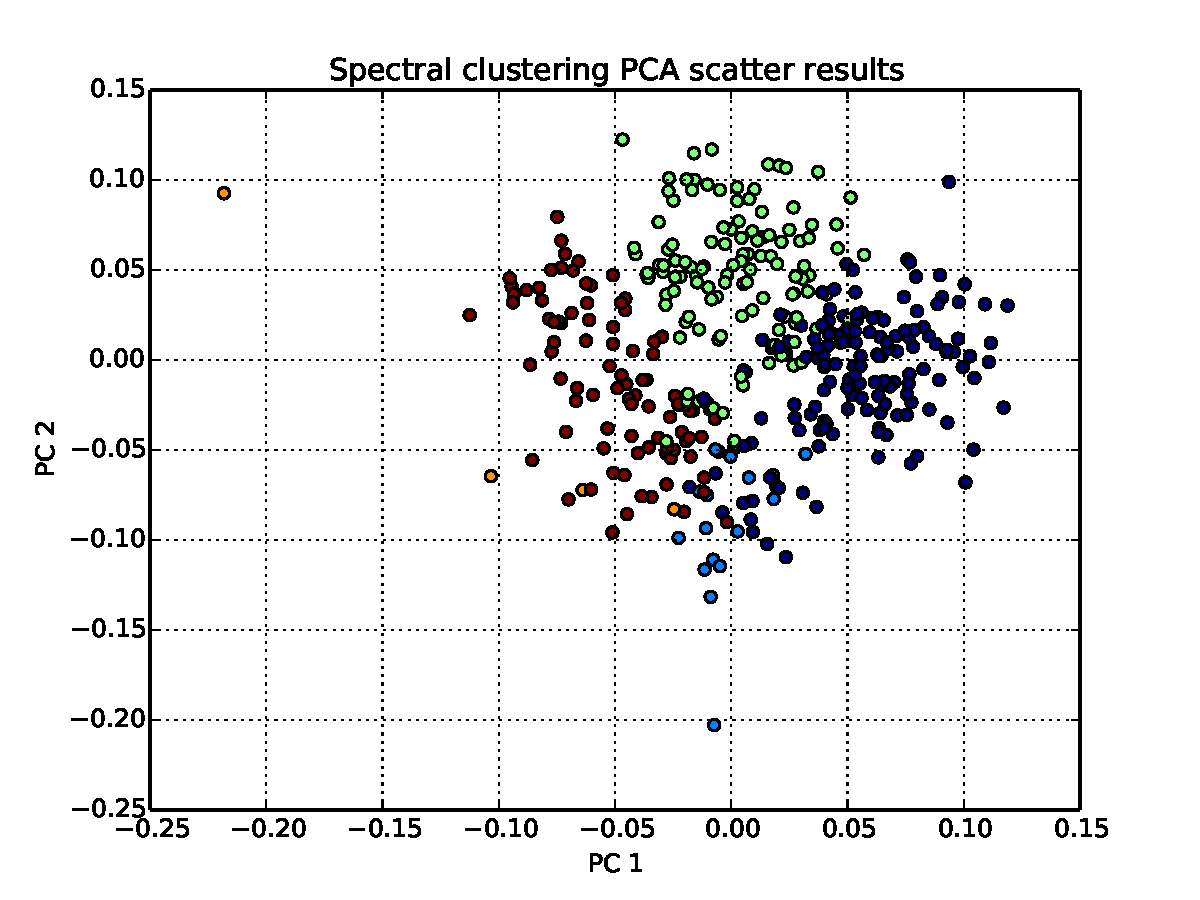
\includegraphics[width=0.8\textwidth]{S_cho_2D.pdf}
	\caption{Result of spectral clustering on Cho DataSet  2D Version, K=5, $\sigma$ = 2}
\end{figure}

\begin{figure}[H]
	\centering
	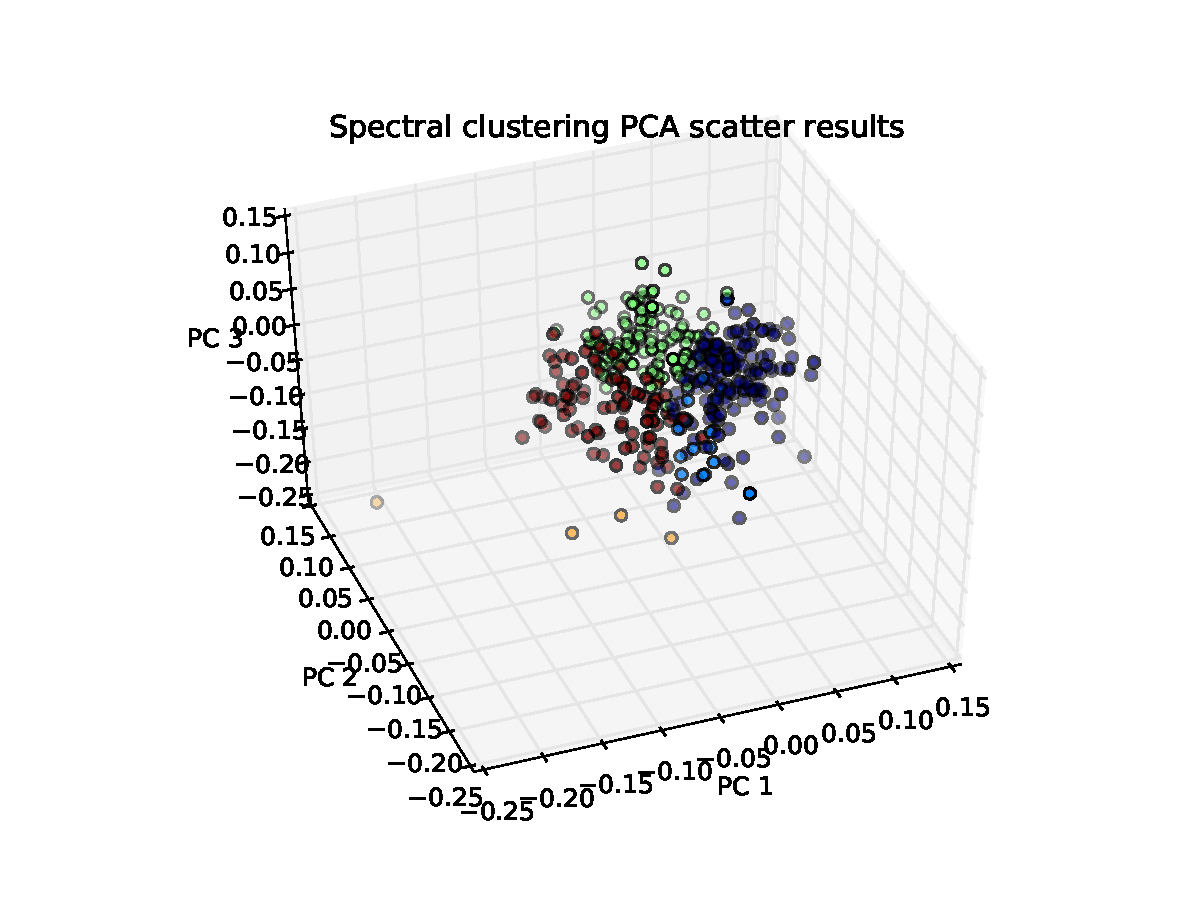
\includegraphics[width=0.8\textwidth]{S_cho_3D.pdf}
	\caption{Result of spectral clustering on Cho DataSet 3D Version, K=5, $\sigma$ = 2}
\end{figure}
\noindent Rand Index = 0.7570\\
Jaccard Coefficient = 0.3817\\


\begin{figure}[H]
	\centering
	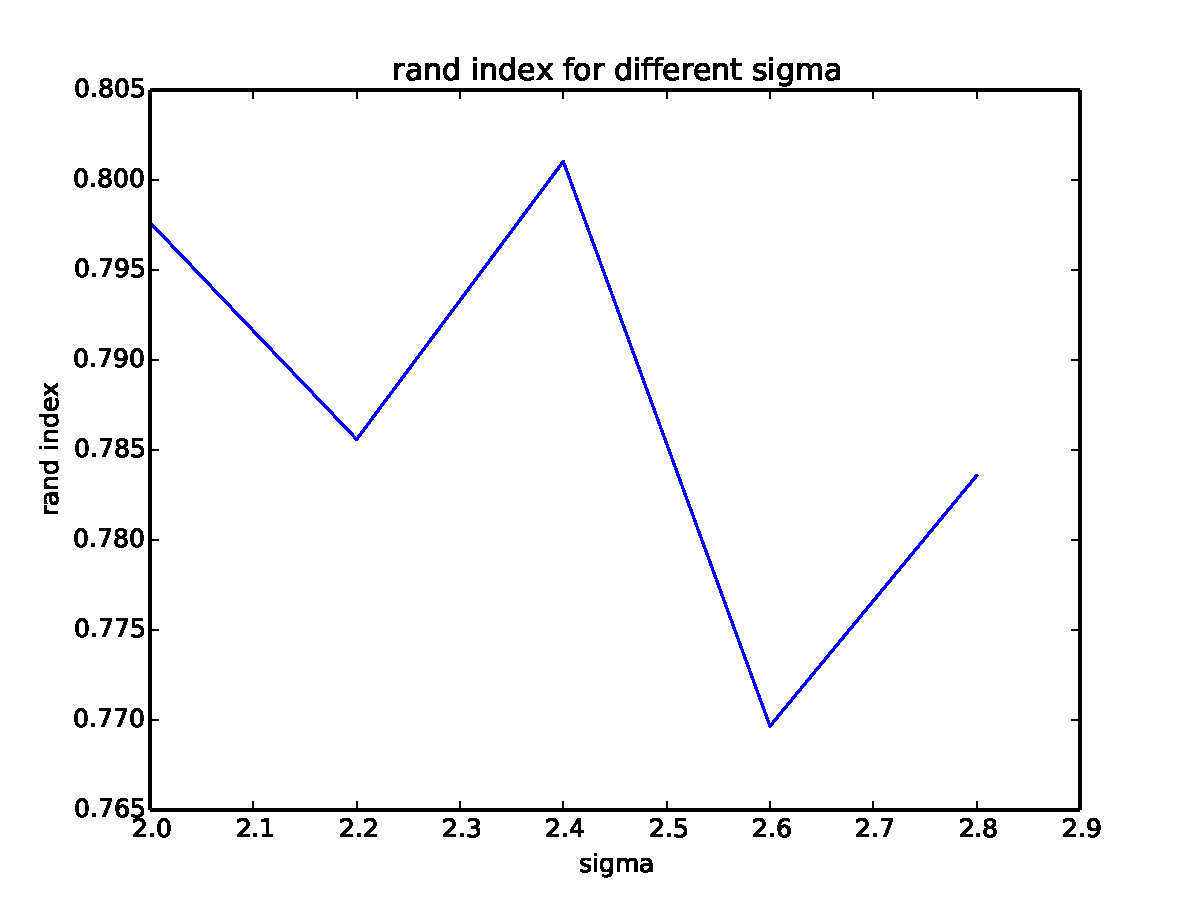
\includegraphics[width=0.8\textwidth]{choose_sigma_iyer.pdf}
	\caption{Choosing $\sigma$ for Iyer DataSet  }
\end{figure}


\begin{figure}[H]
	\centering
	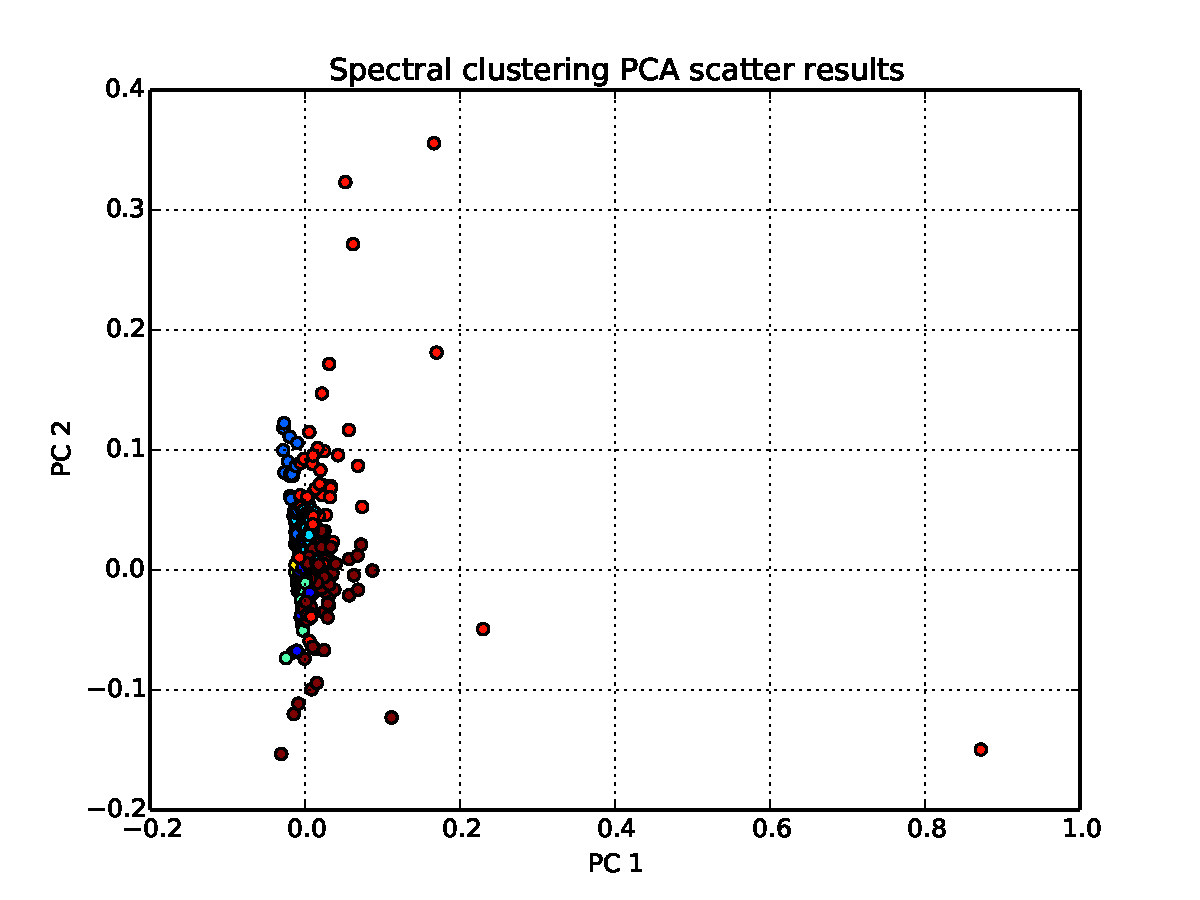
\includegraphics[width=0.8\textwidth]{S_iyer_2D.pdf}
	\caption{Result of spectral clustering on iyer DataSet  2D Version, K=10, $\sigma$ = 2.4}
\end{figure}

\begin{figure}[H]
	\centering
	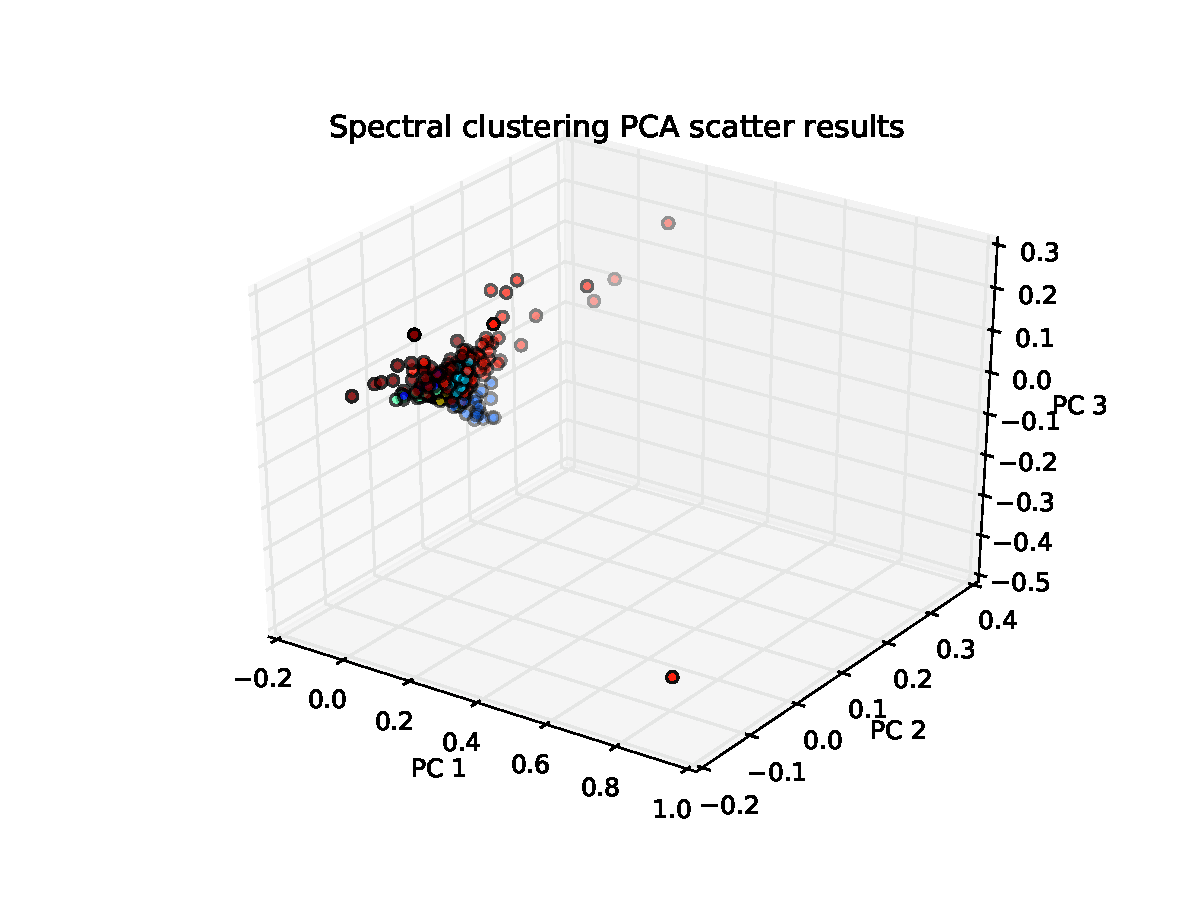
\includegraphics[width=0.8\textwidth]{S_iyer_3D.pdf}
	\caption{Result of spectral clustering on iyer DataSet 3D Version, K=10, $\sigma$ = 2.4}
\end{figure}
\noindent Rand Index = 0.8241\\
Jaccard Coefficient = 0.2742\\


\begin{figure}[H]
	\centering
	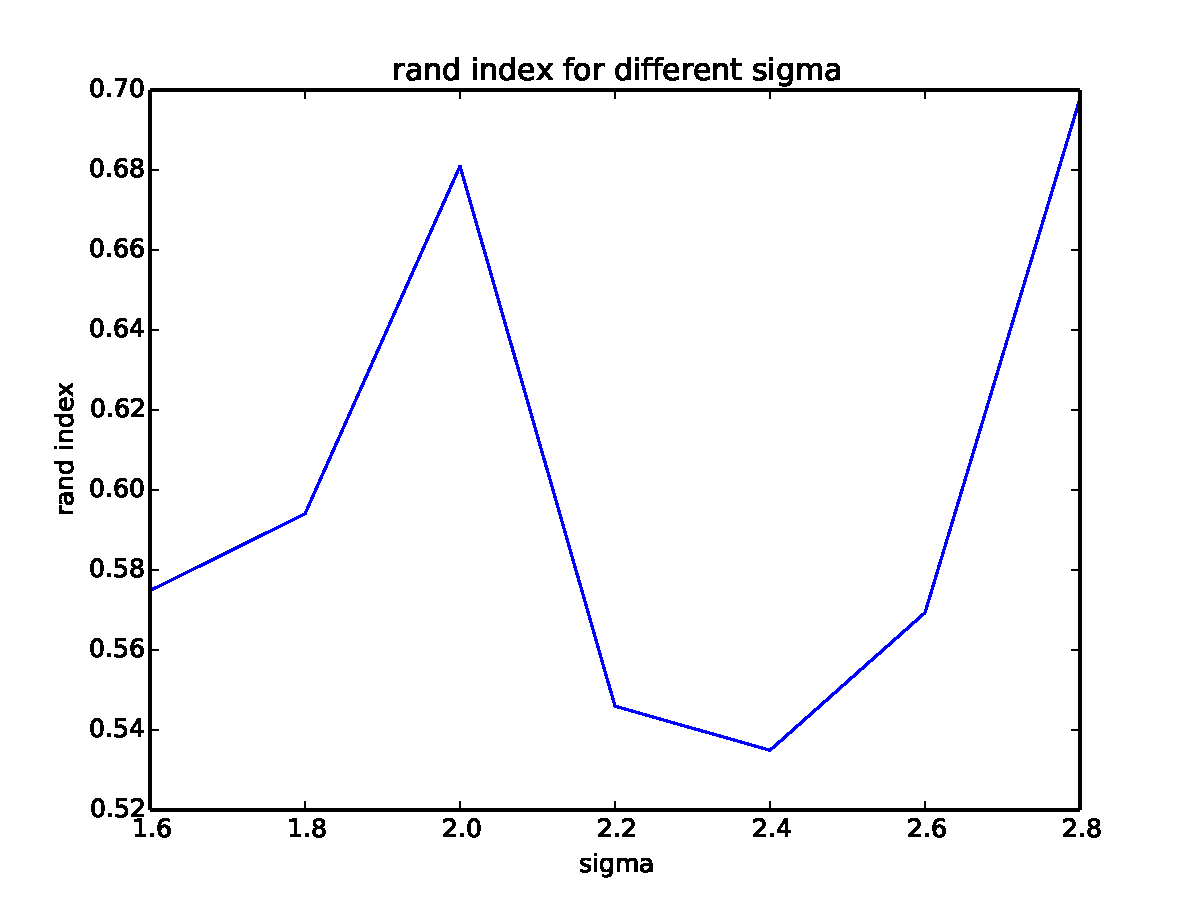
\includegraphics[width=0.8\textwidth]{choose_sigma_new_dataset1.pdf}
	\caption{Choosing $\sigma$ for new DataSet 1 }
\end{figure}


\begin{figure}[H]
	\centering
	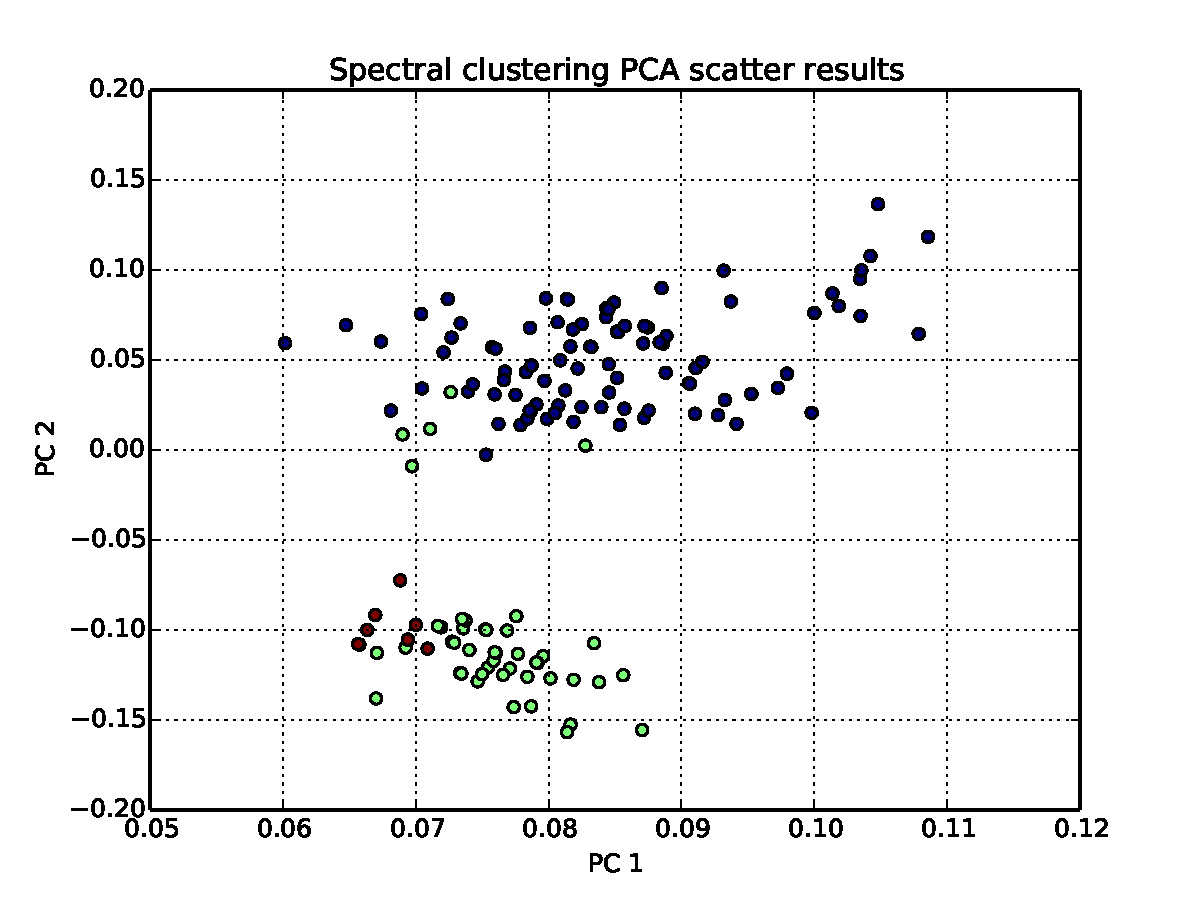
\includegraphics[width=0.8\textwidth]{S_new_dataset_1_2D.pdf}
	\caption{Result of spectral clustering on new DataSet 1 2D Version, K=3, $\sigma$ = 2.8}
\end{figure}

\begin{figure}[H]
	\centering
	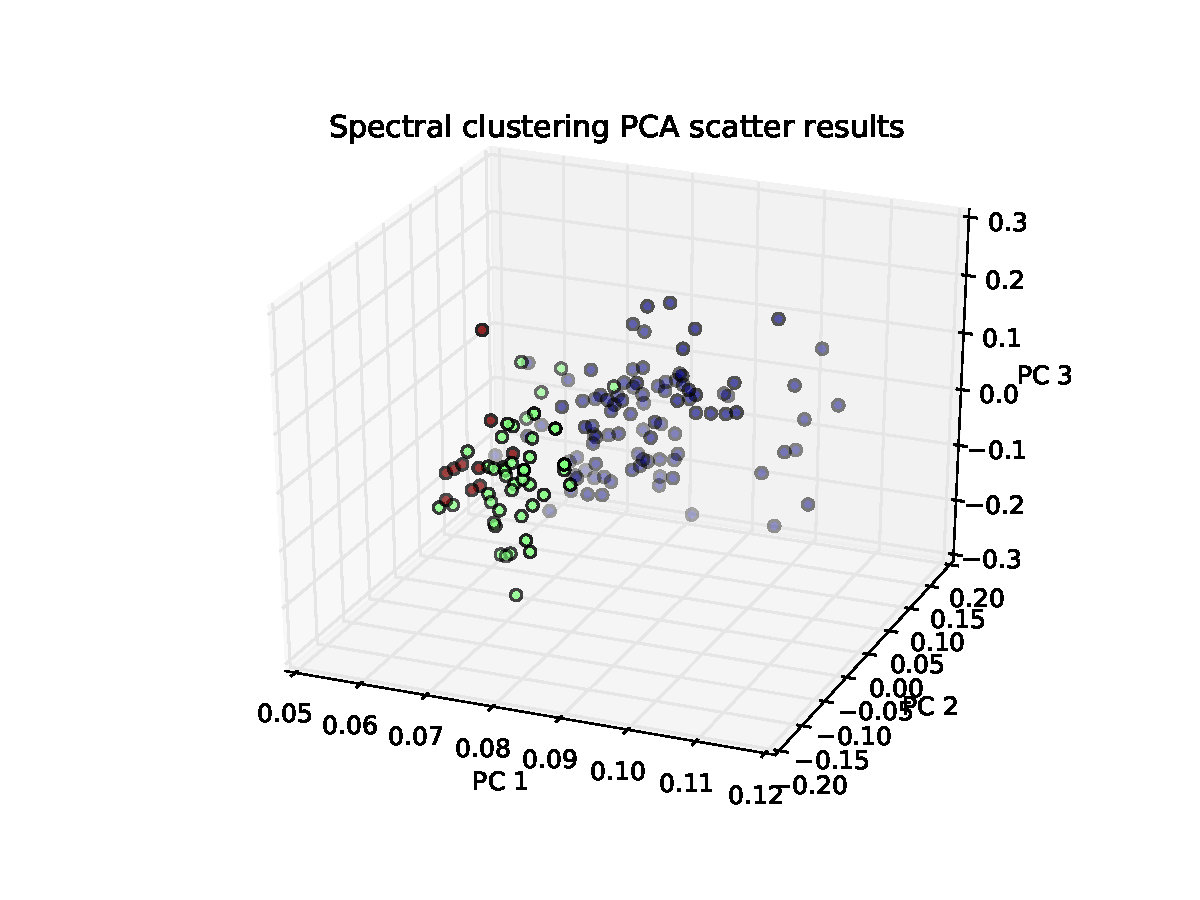
\includegraphics[width=0.8\textwidth]{S_new_dataset_1_3D.pdf}
	\caption{Result of spectral clustering on new DataSet 1 3D Version, K=3, $\sigma$ = 2.8}
\end{figure}
\noindent Rand Index = 0.7267\\
Jaccard Coefficient = 0.5040\\




\begin{figure}[H]
	\centering
	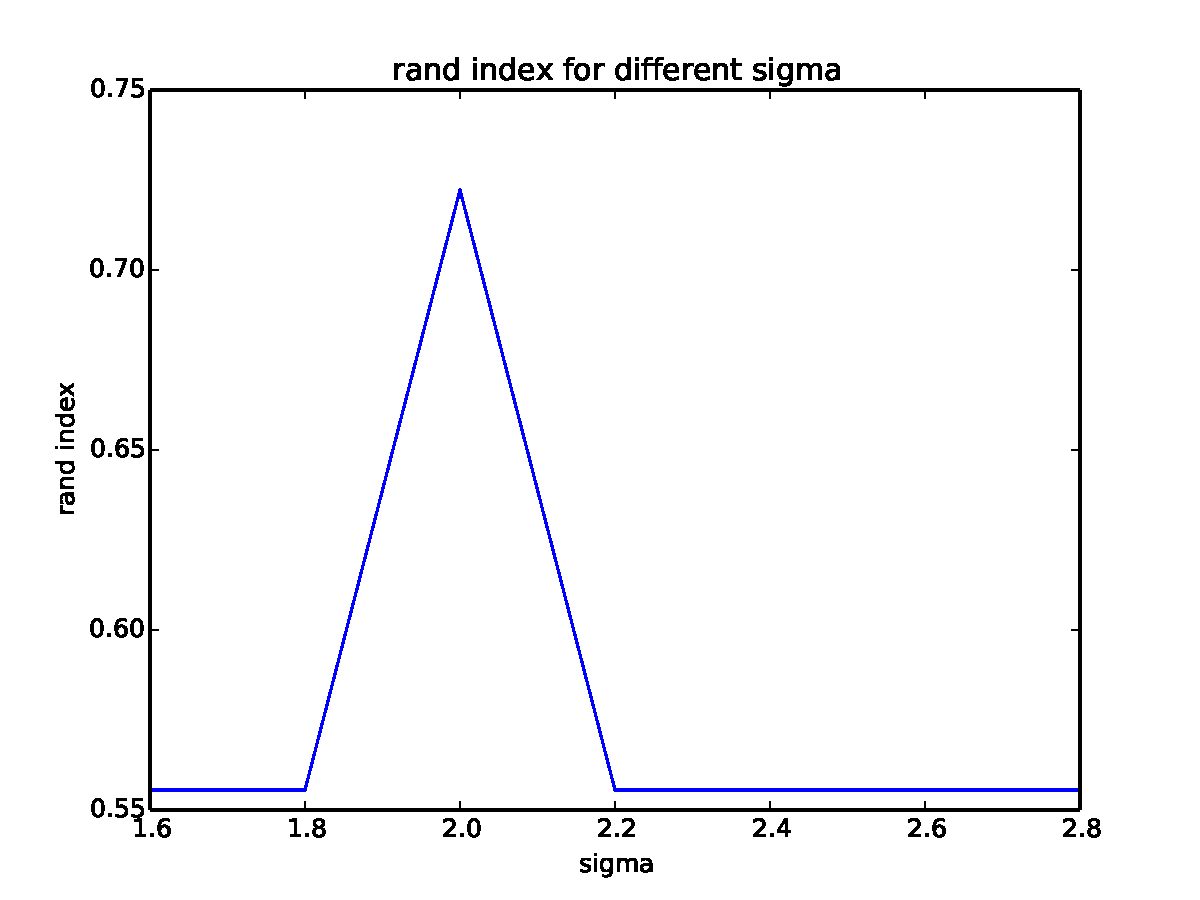
\includegraphics[width=0.8\textwidth]{choose_sigma_new_dataset2.pdf}
	\caption{Choosing $\sigma$ for new DataSet 2 }
\end{figure}


\begin{figure}[H]
	\centering
	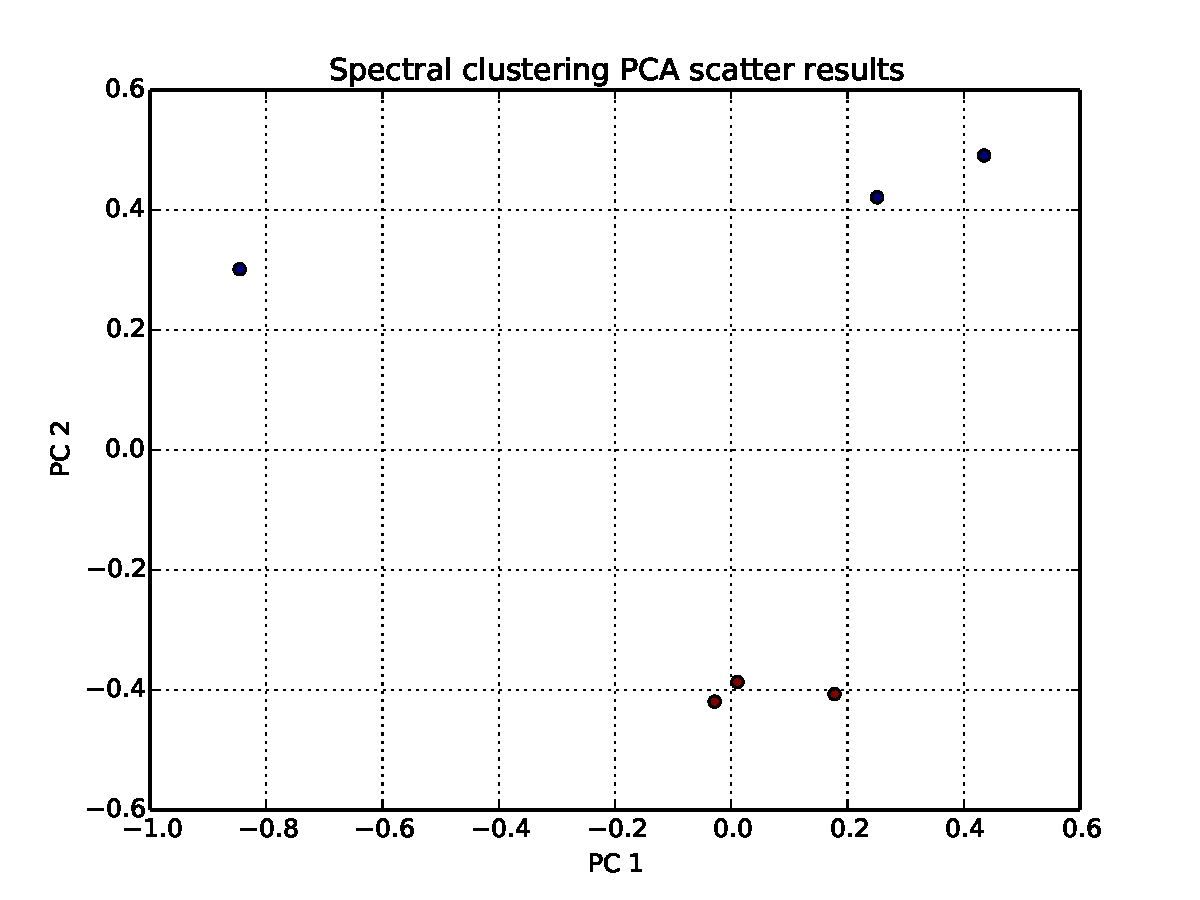
\includegraphics[width=0.8\textwidth]{S_new_dataset_2_2D.pdf}
	\caption{Result of spectral clustering on new DataSet 2 2D Version, K=2, $\sigma$ = 2}
\end{figure}

\begin{figure}[H]
	\centering
	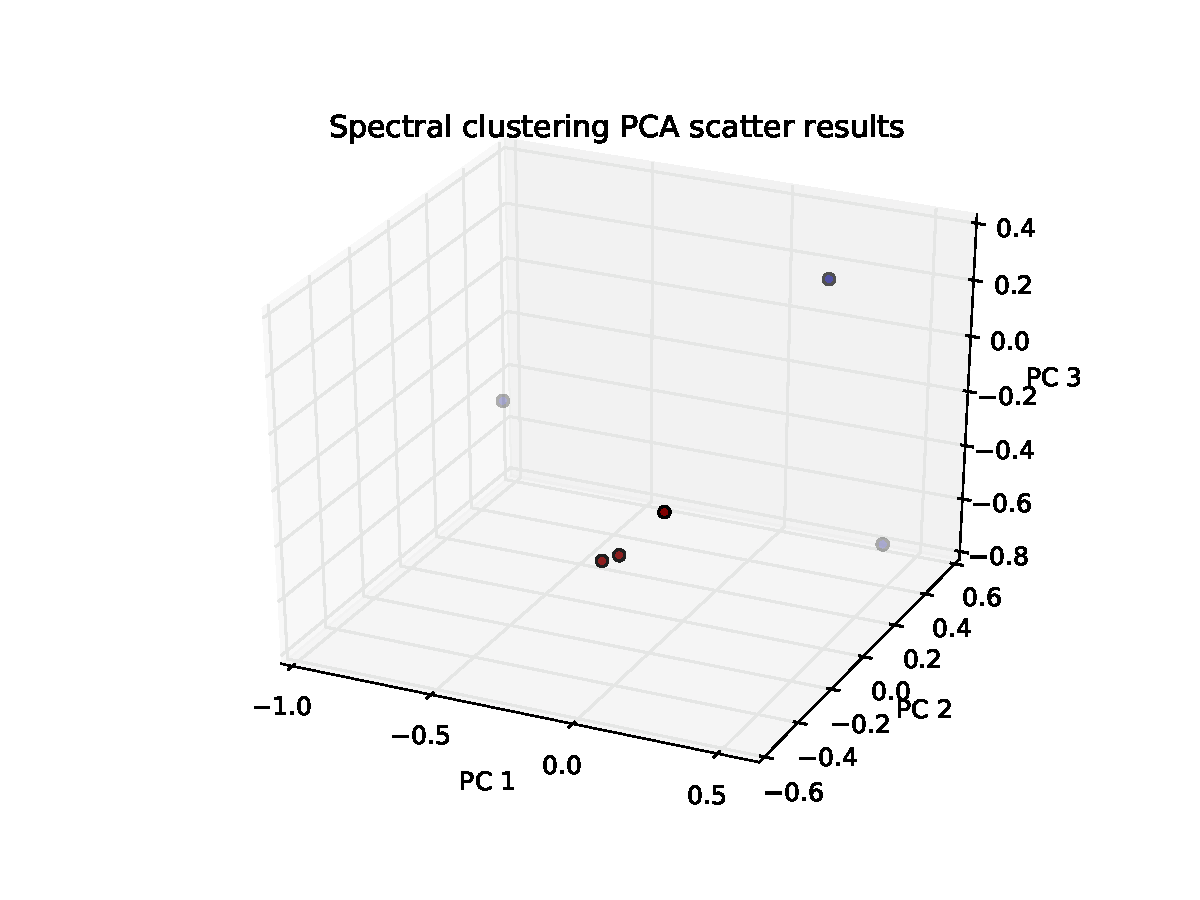
\includegraphics[width=0.8\textwidth]{S_new_dataset_2_3D.pdf}
	\caption{Result of spectral clustering on new DataSet 2 3D Version, K=2, $\sigma$ = 2}
\end{figure}
\noindent Rand Index = 1.0000\\
Jaccard Coefficient = 1.0000\\

\subsection{Result Evaluation}
Spectral clustering is built on beautiful mathematics and the solution is elegant, which has a closed form. But it's not very robust to noise, like for iyer dataset, which has some outliers, its performance is badly affected. Another drawback is it will become computationally expensive if the input dimension gets large because of the computation for eigen values and eigen vectors.

\subsection{Algorithm Description}
Kmeans is a nice algorithm to implement with map reduce because it is embarrassingly parallel. Kmeans consists of calculating the distance of a node with every centroid, finding the centroid which has the minimum distance, assigning each entry to a cluster and then updating the centroids. It is clear that calculating the distances between nodes and centroids can be done independently from other nodes. Therefore, this can be our map function that can be performed in parallel. Our reduce function would contain finding the minimum, assigning the node to a new centroid and calculating the new centroid. This is identical to the Kmeans described above, but in this part of the project we take advantage of the fact that kmeans is embarrassingly parallel.
\subsection{Implementation}
For this project, we used Hadoop to implement MapReduce Kmeans. We used hadoop streaming to read lines in from our data file to our mapper file, and then also used streaming to read in the outputs from the mapper file to the reducer program. In the mapper program, we calculated the distance of a node x and all k centroids. We then printed x's ID and its distances. In the sequential implementation of kmeans, we are not concerned with the ID because there is only one process running and you know exactly what order things are being run in. However, in the parallel version of kmeans, we have to keep track of x's ID because there are multiple distances being calculated at the same time. Simply printing out the distances would not be sufficient because we would not know which node this corresponds to. \\

In our reduce, we take in these values and also read in from a cached file which tells us the current centroids. We calculate the minimum distance becaused on the distances already given to us, and then assign each node x to a new centroid (if necessary). We know that we have finished assigning all nodes when we stop receiving inputs from the mapper program. Once this happens, we calculate the new centroids by calculating the average distance between each node and assigning that as the centroid. This is then updated in our cache file. We are also constantly updating another file which stores all current assignments of the nodes. 

For this project, I wrote a script to repeatly call map and reduce. In the script, I specify the number of iterations of map and reduce to be performed. We can do multiple iterations because in each iteration, the centroids are updated. In the ideal scenerio, our program would converge within the number of iterations we allow it. Fortunately for this project, the datasets were relatively small so we are typically able to converge within 20 iterations. However, if we don't converge within the given iterations, we still have the assignments for the first 20 iterations. With this, we can visualize the state of our program at the 20th iteration.
\subsection{Result Visualization}
\begin{figure}[H]
	\centering
	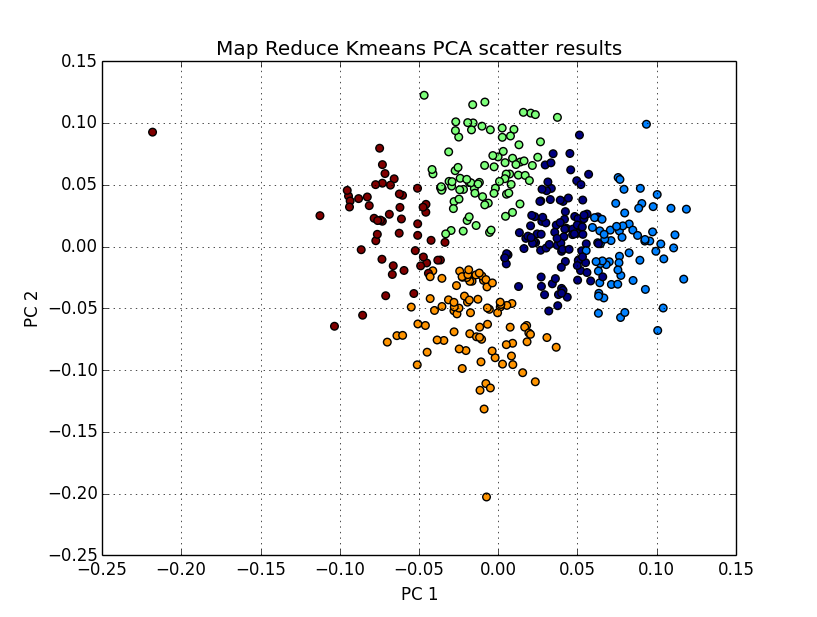
\includegraphics[width=0.8\textwidth]{MP_cho_2D}
	\caption{Result of K\_Means Map Reduce Algorithm on Cho DataSet 2D Version, K=5}
\end{figure}
\begin{figure}[H]
	\centering
	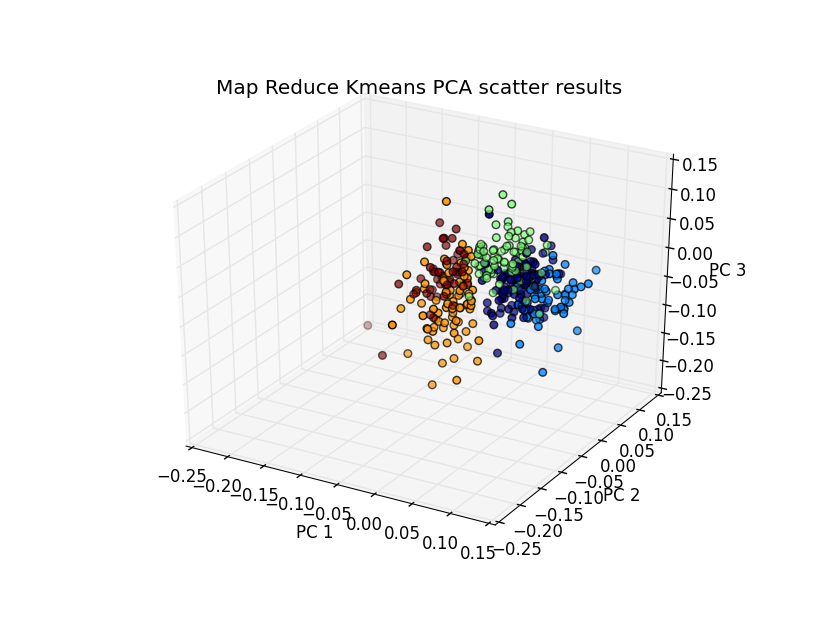
\includegraphics[width=0.8\textwidth]{MP_cho_3D}
	\caption{Result of K\_Means Map Reduce Algorithm on Cho DataSet 3D Version, K=5}
\end{figure}
\begin{figure}[H]
	\centering
	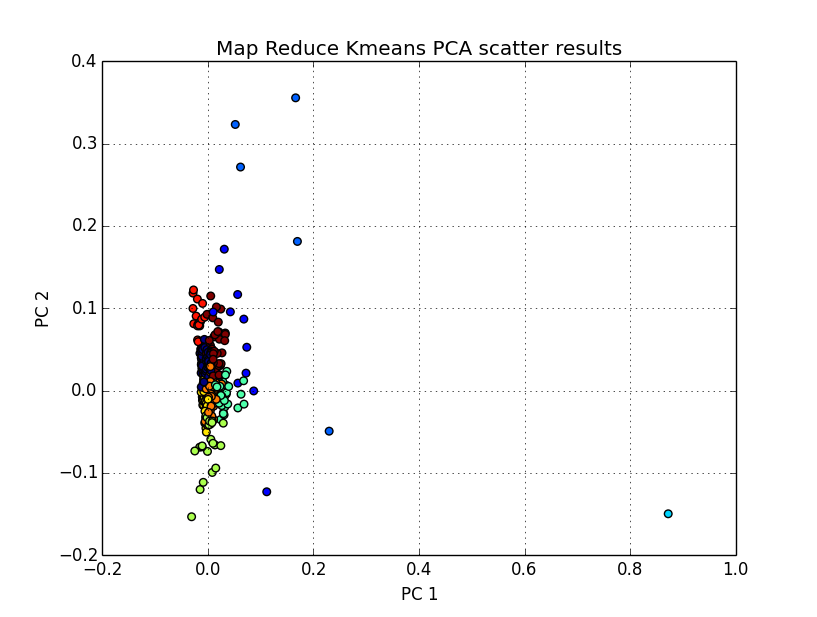
\includegraphics[width=0.8\textwidth]{MP_iyer_2D}
	\caption{Result of K\_Means Map Reduce Algorithm on Iyer DataSet 2D Version,K=10}
\end{figure}
\begin{figure}[H]
	\centering
	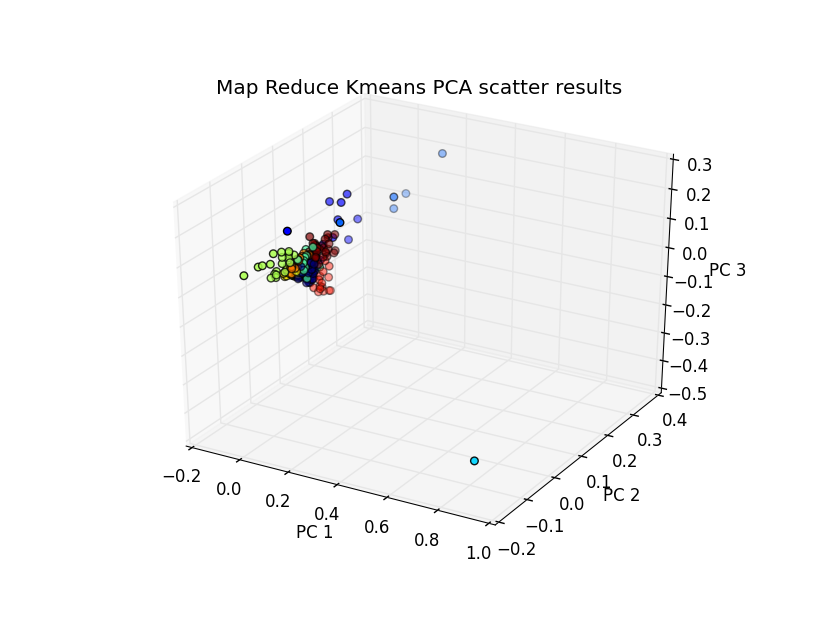
\includegraphics[width=0.8\textwidth]{MP_iyer_3D}
	\caption{Result of K\_Means Map Reduce Algorithm on Iyer DataSet 3D Version,K=10}
\end{figure}
\begin{figure}[H]
	\centering
	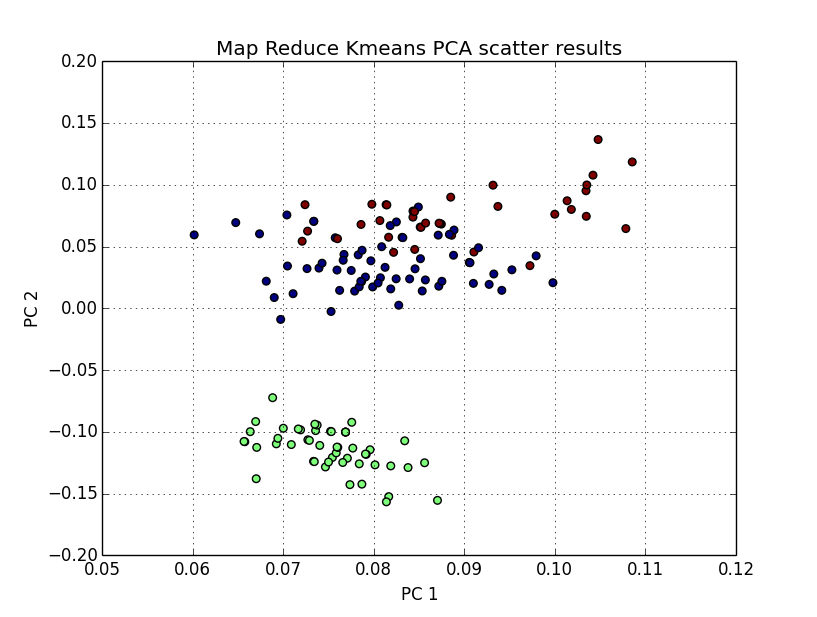
\includegraphics[width=0.8\textwidth]{MP_new_dataset_1_2D}
	\caption{Result of K\_Means Map Reduce Algorithm on new dataset 1 DataSet 2D Version,K=3}
\end{figure}
\begin{figure}[H]
	\centering
	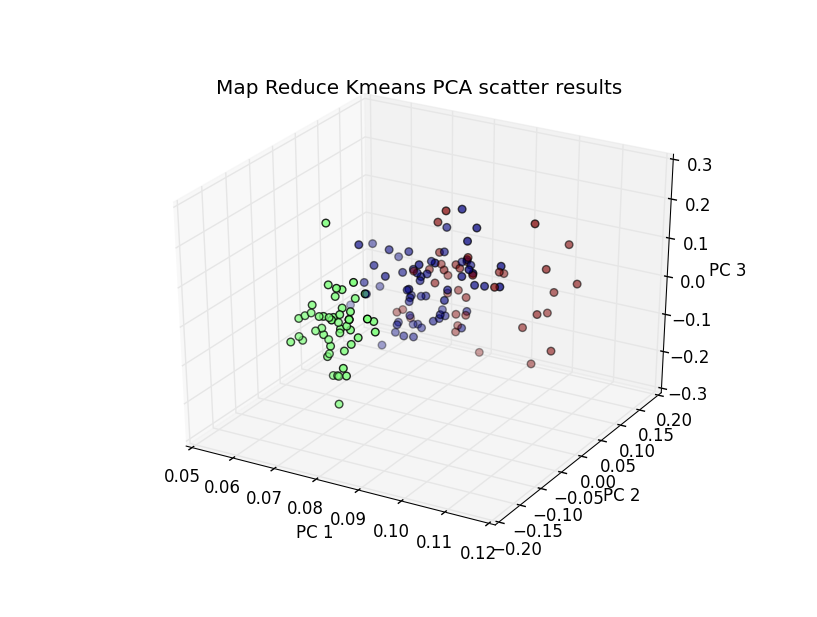
\includegraphics[width=0.8\textwidth]{MP_new_dataset_1_3D}
	\caption{Result of K\_Means Map Reduce Algorithm on new dataset 1 DataSet 3D Version,K=3}
\end{figure}
\begin{figure}[H]
	\centering
	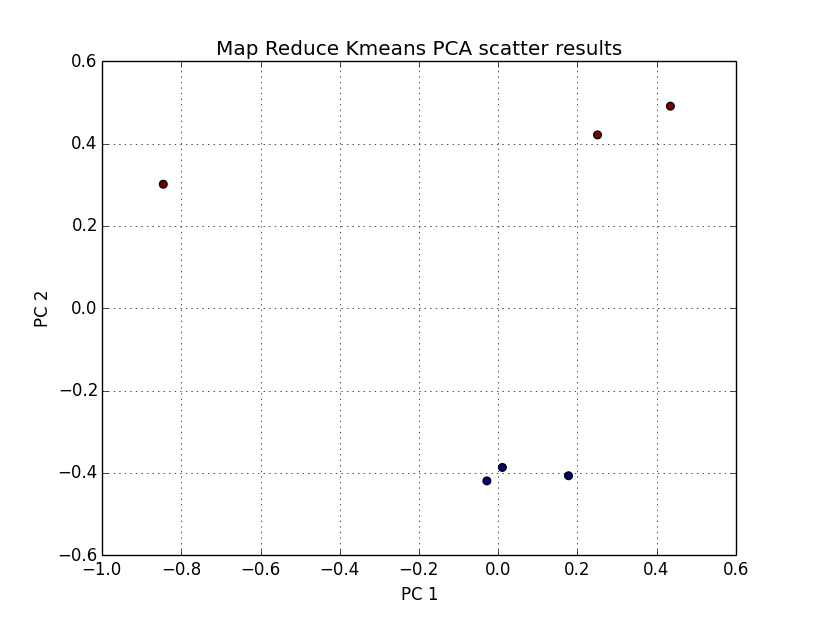
\includegraphics[width=0.8\textwidth]{MP_new_dataset_2_2D}
	\caption{Result of K\_Means Map Reduce Algorithm on new dataset 2 DataSet 2D Version,K=2}
\end{figure}
\begin{figure}[H]
	\centering
	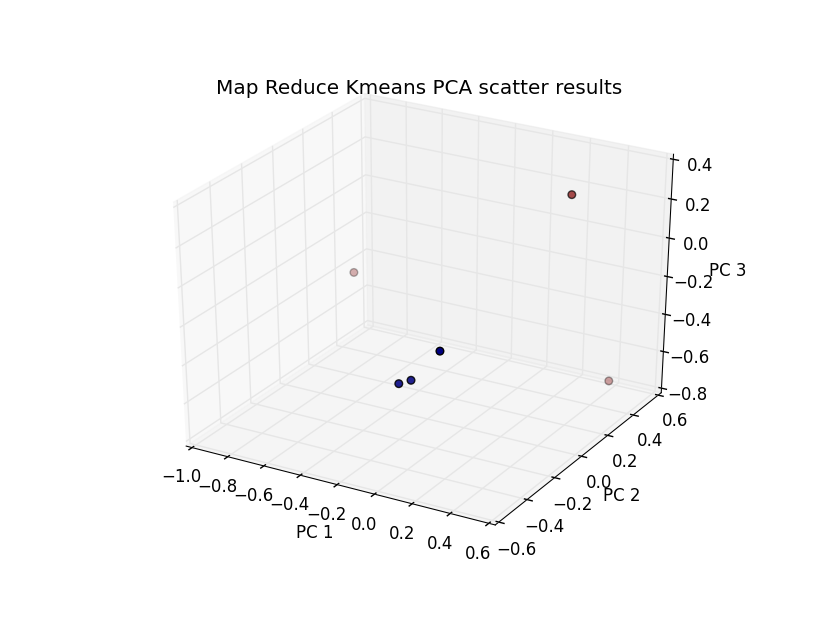
\includegraphics[width=0.8\textwidth]{MP_new_dataset_2_3D}
	\caption{Result of K\_Means Map Reduce Algorithm on new dataset 2 DataSet 3D Version,K=2}
\end{figure}
\subsection{Result Evaluation}
The map reduce kmeans has the same strong and weak points as the sequentially implemented kmeans described earlier. An additional downside to mapreduce kmeans, however, is that it runs more slowly than the sequentially kmeans. This is because of the overhead cost of using hadoop and setting up our node. The map reduce kmeans would likely outperform the sequential kmeans for large datasets, but the datasets we were given for this assignment were relatively small. 
\begin{thebibliography}{1}
\bibitem{sp_clustering}
Ng, Andrew Y., Michael I. Jordan, and Yair Weiss. "On spectral clustering: Analysis and an algorithm." Advances in neural information processing systems 2 (2002): 849-856.
\end{thebibliography}


\end{document}